\documentclass[a4paper]{article}

%% Language and font encodings
\usepackage[english]{babel}
\usepackage[utf8x]{inputenc}
\usepackage[T1]{fontenc}
\usepackage{pdfpages}
\usepackage{float}

%% Sets page size and margins
\usepackage[a4paper,top=3cm,bottom=2cm,left=3cm,right=3cm,marginparwidth=1.75cm]{geometry}

%% Useful packages
\usepackage{amsmath}
\usepackage{graphicx}
\usepackage[colorinlistoftodos]{todonotes}
\usepackage[colorlinks=true, allcolors=blue]{hyperref}

%% to import csv table
\usepackage{csvsimple}

\title{M2 EEE: Financial Econometrics - Homework 1 \footnote{The R source code for replication all results in this paper is available at \url{https://github.com/maianhdang/garch_VaR} }}
\author{Mai-Anh Dang | Student ID: 21608631 \\
Hoang Tran | Student ID: 21208337 }

\begin{document}
\maketitle


\section{Descriptive statistics of financial data}
\subsection{Sample Statistics}

\paragraph{}
In the \textbf{Table \ref{tab:sample-stat}} below, we present some sample statistics of Spyder daily Return, Squared Return and Realized Volatility. As can be seen, the Skewness of Daily Return is 0.0147, which means we have a relatively balanced distribution of return with a slight positive skewness. This skewness of return indicates that Spyder performs relatively well, with probability obtaining negative results is low. The Skewness for Squared (Sqd.) Return and RV is quite high, which is unsurprising since both indexes is related to the volatility (squared variance of the return) and strictly positive.\\

Regarding kurtosis, the value for Spyder daily return is 10.69967, which is strictly greater than 3 of normal distribution. It suggests that Spyder is also a risky asset, as it has a great amount of returns distributed at its tails, and its investors face high probability of having extreme loss. Kurtosis of Squared Return and RV once again significantly higher than Return.\\

Standard Deviation of Return is 0.0126, which dominates its mean of 0.0002. This results is in line with Empirical Stylized Fact about short horizon return such as daily frequency. The Standard Deviation of Return is also significantly higher than of Squared Return (0.0005) and Realized Volatility (0.0003).

%------------ Table: Sample Statistics -----------------%

\begin{table}[H] \centering 
  \caption{Sample Statistics} 
  \label{tab:sample-stat} 
\begin{tabular}{@{\extracolsep{4pt}} cccc} 

\\[-1.8ex]\hline 
\hline \\[-1.8ex] 
 
\\[-1.8ex] & Return & Sqd. Return & RV 
\\ 
 & (1) & (2) & (3) \\ % Column 1 is OK, we need to fill column 2, 2B, 2C
\hline \\[-1.8ex] 
Mean & 0.0002 &  1.588e-04 & 9.950e-05 \\[1.8ex]

Variance & 0.0001 & 3.2037e-07 & 0.0000 \\ [1.8ex]

Std. Dev & 0.0126 & 0.0005 & 0.0003 \\ [1.8ex]

Skewness & 0.0147 & 12.2202 & 10.2890  \\ [1.8ex]

Kurtosis & 10.69967 & 215.334 & 161.1583 \\[1.8ex]

\hline \\[-1.8ex] 

\end{tabular} 
\end{table} 
%-----------------------------------%

\paragraph{}
From \textbf{Figure \ref{fig:acf1_plot}}, we can obtain the ACF of Return, Squared Return and Realized Volatility. There are still exist serial correlation in Spyder daily return at 1-2 lags but it decays rapidly, afterwards the magnitude is relatively low. This result is in line with Stylized Fact of daily return, which stated that daily return have very little autocorrelation, and it is almost impossible to predict from their own past. Squared Return and Realized Volatility both demonstrates a significantly strong and positive correlation with their own past. This is the evidence that the squared return is not the process of i.i.d random variable. On the other hand, we expect that past squared returns could contribute to predict subsequent ones. It is similar to realized volatility, which is the proxy for unobservable variance of returns. This motivates us to apply GARCH models later to model the volatility. \\ 

\textbf{In all graphs, the series is represented by time index/period from t=1 ("2004-06-15") to t=2,497 ("2014-06-13")}.
Considering the Time series of Return, Squared Return and RV, we can observe some intense volatility at the time index from t = 1,000 ("2008-06-13") to t = 1,200 ("2009-04-03"). This period correspond to the Financial crisis (from 2008 to 2009), so the volatility is larger than other periods. One can also see the pattern that the large volatility today would be more likely followed by a large volatility tomorrow, and vice versa.


\begin{figure}[H]
\centering
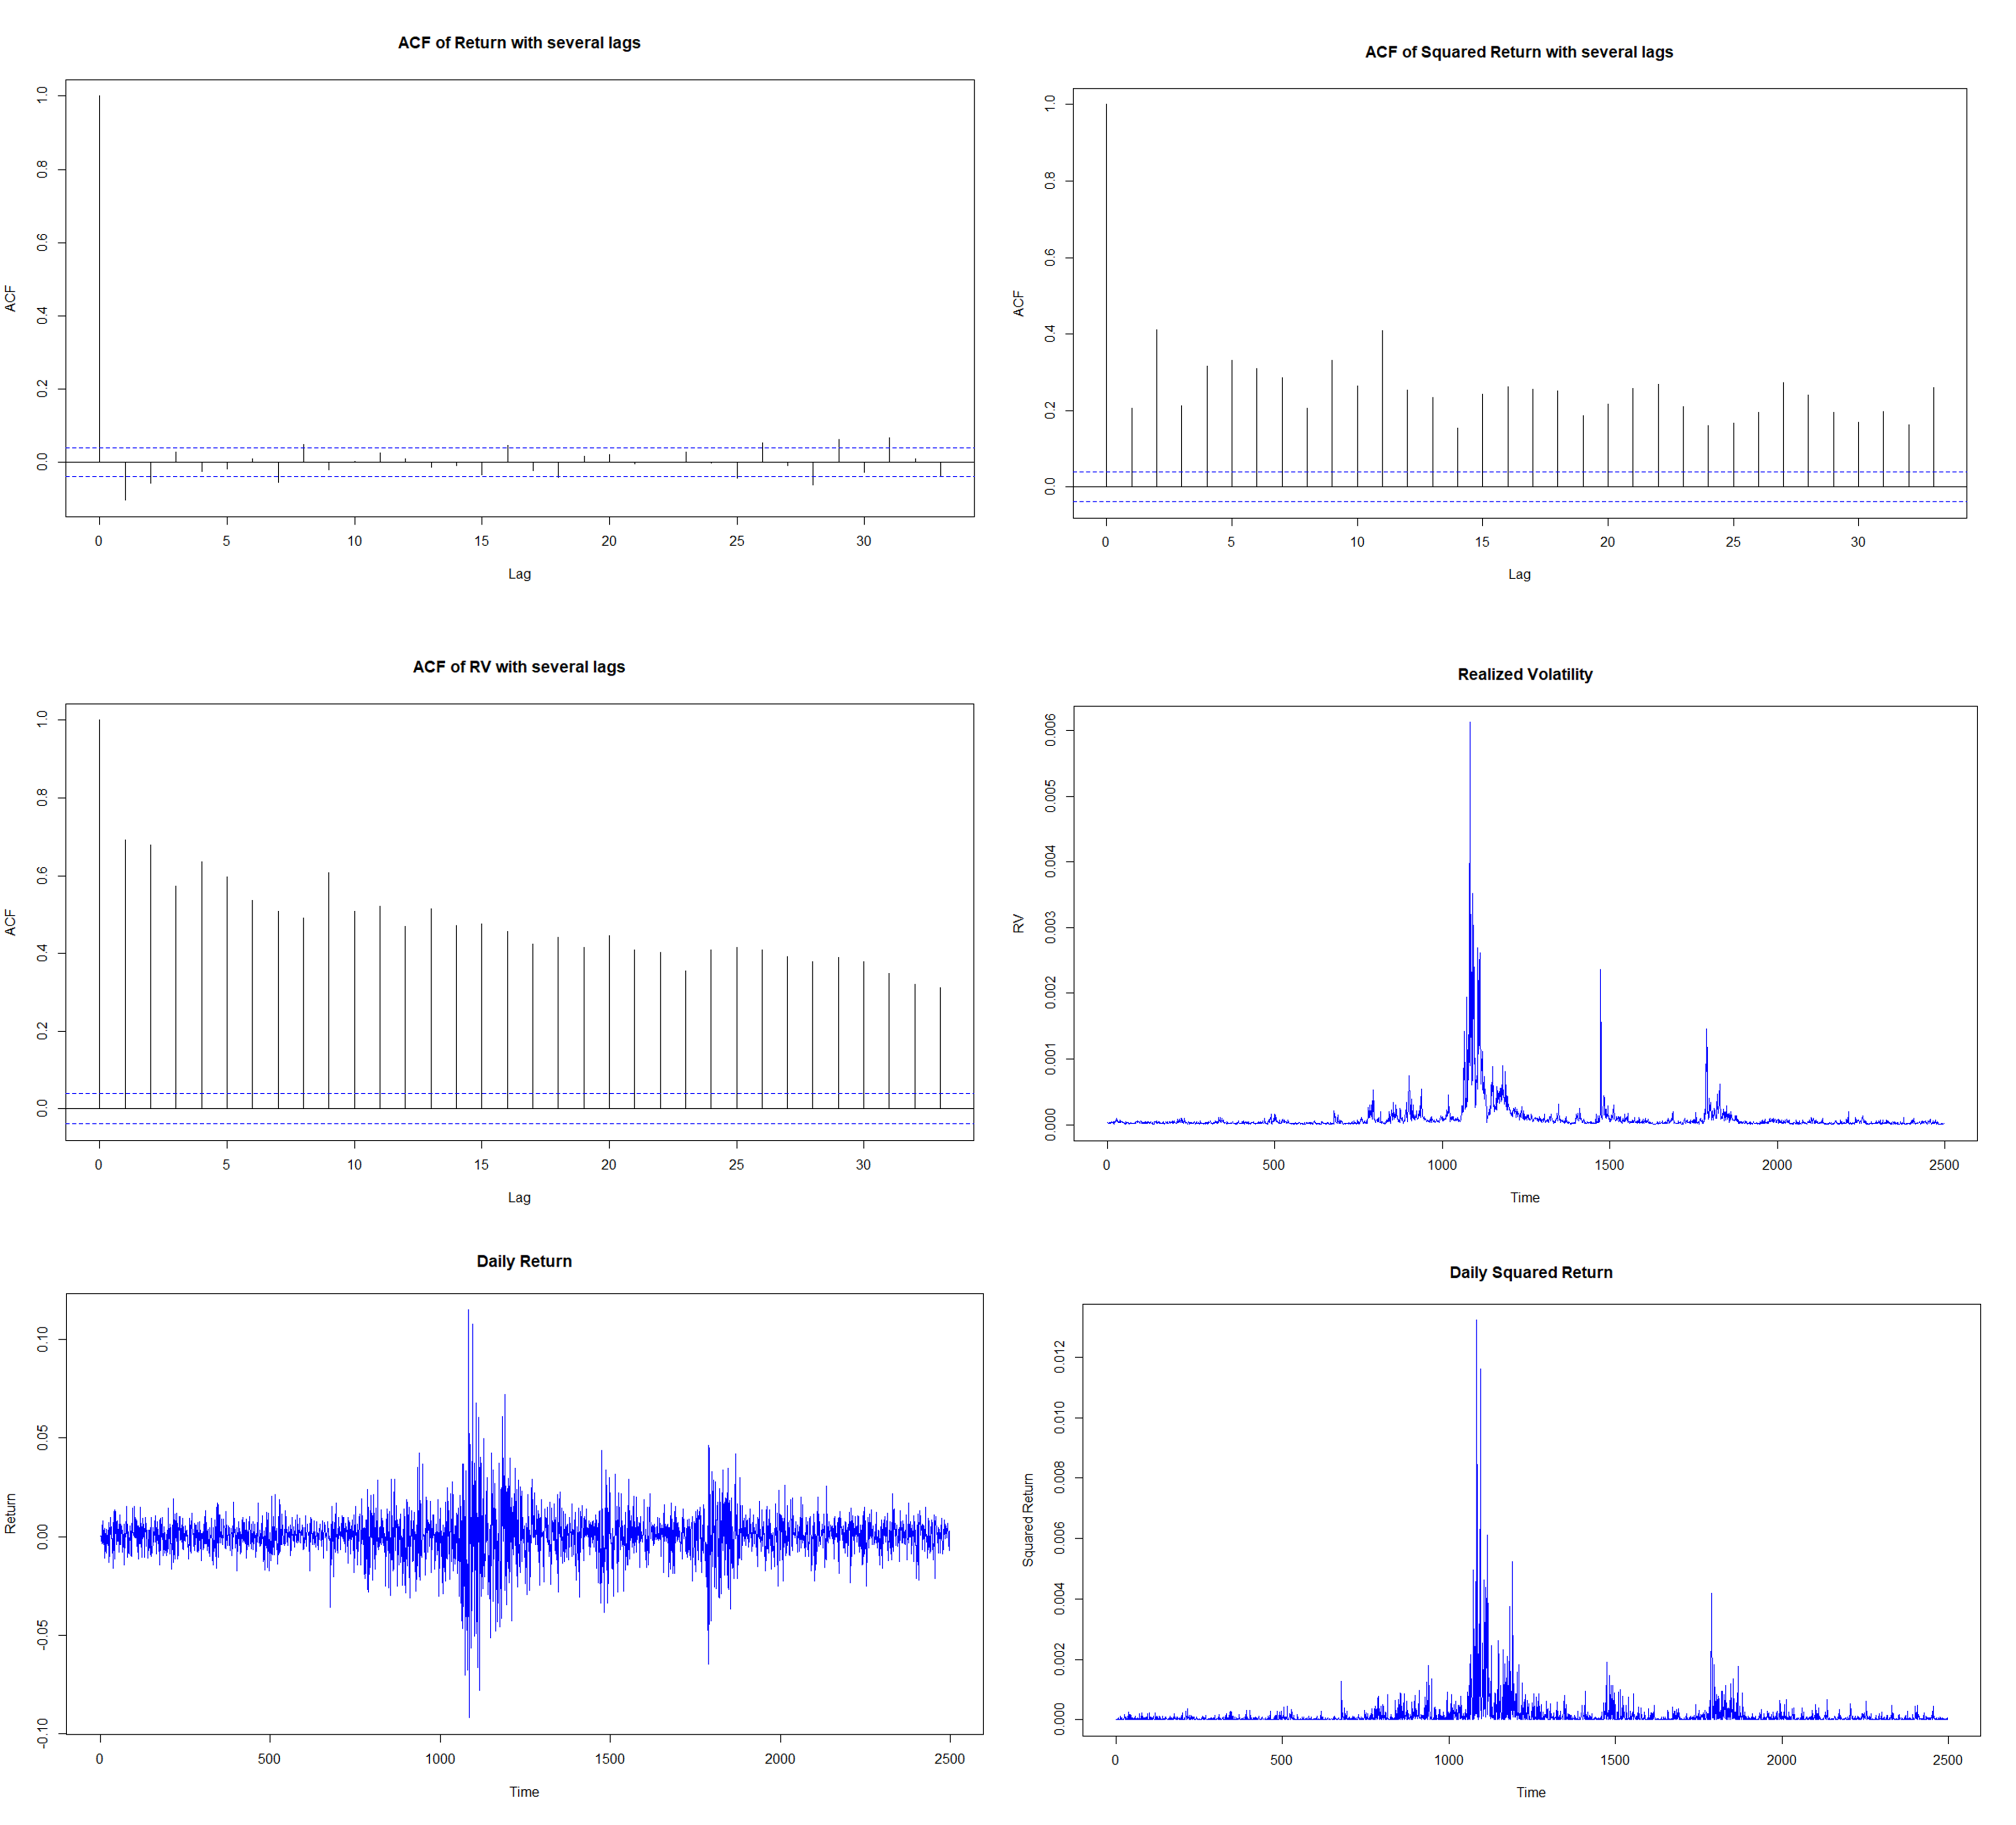
\includegraphics[width=1.05\textwidth]{AF2.png}
\caption{\label{fig:acf1_plot}Plot of Return, Squared Return, RV and its ACF}
\end{figure}

\subsection{Rolling Statistics}
\paragraph{}
Rolling Statistics is a method to investigate the evolution of a statistics through time. For this data, we have considered several window size: In fact, large window size would lead to overly smooth, while to small window sizes make the graphs with over 2,000 time observations difficult to see. We finally choose a window equal to 120 time-periods, which is roughly 4 months as it is smooth enough to easily observe the trends. The rolling statistics of Return and RV is presented in \textbf{Figure \ref{fig:roll-ret} and \ref{fig:roll-rv}.} From \textbf{Figure \ref{fig:roll-ret}}, we can see that the mean begin quite stable, until it plunge to its bottom at the Financial crisis period before recovery months after. The mean continue fluctuating intensively before becoming stable again recently. The same phenomenon for rolling variance as it has its peak during the financial crisis, and be come stable in other periods. Rolling skewness and kurtosis indicates that during sensitive period like financial crisis, it is very likely that investors will face a big loss, as the skewness is strictly negative and kurtosis is significantly greater than 3 at that time.

\begin{figure}[H]
\centering
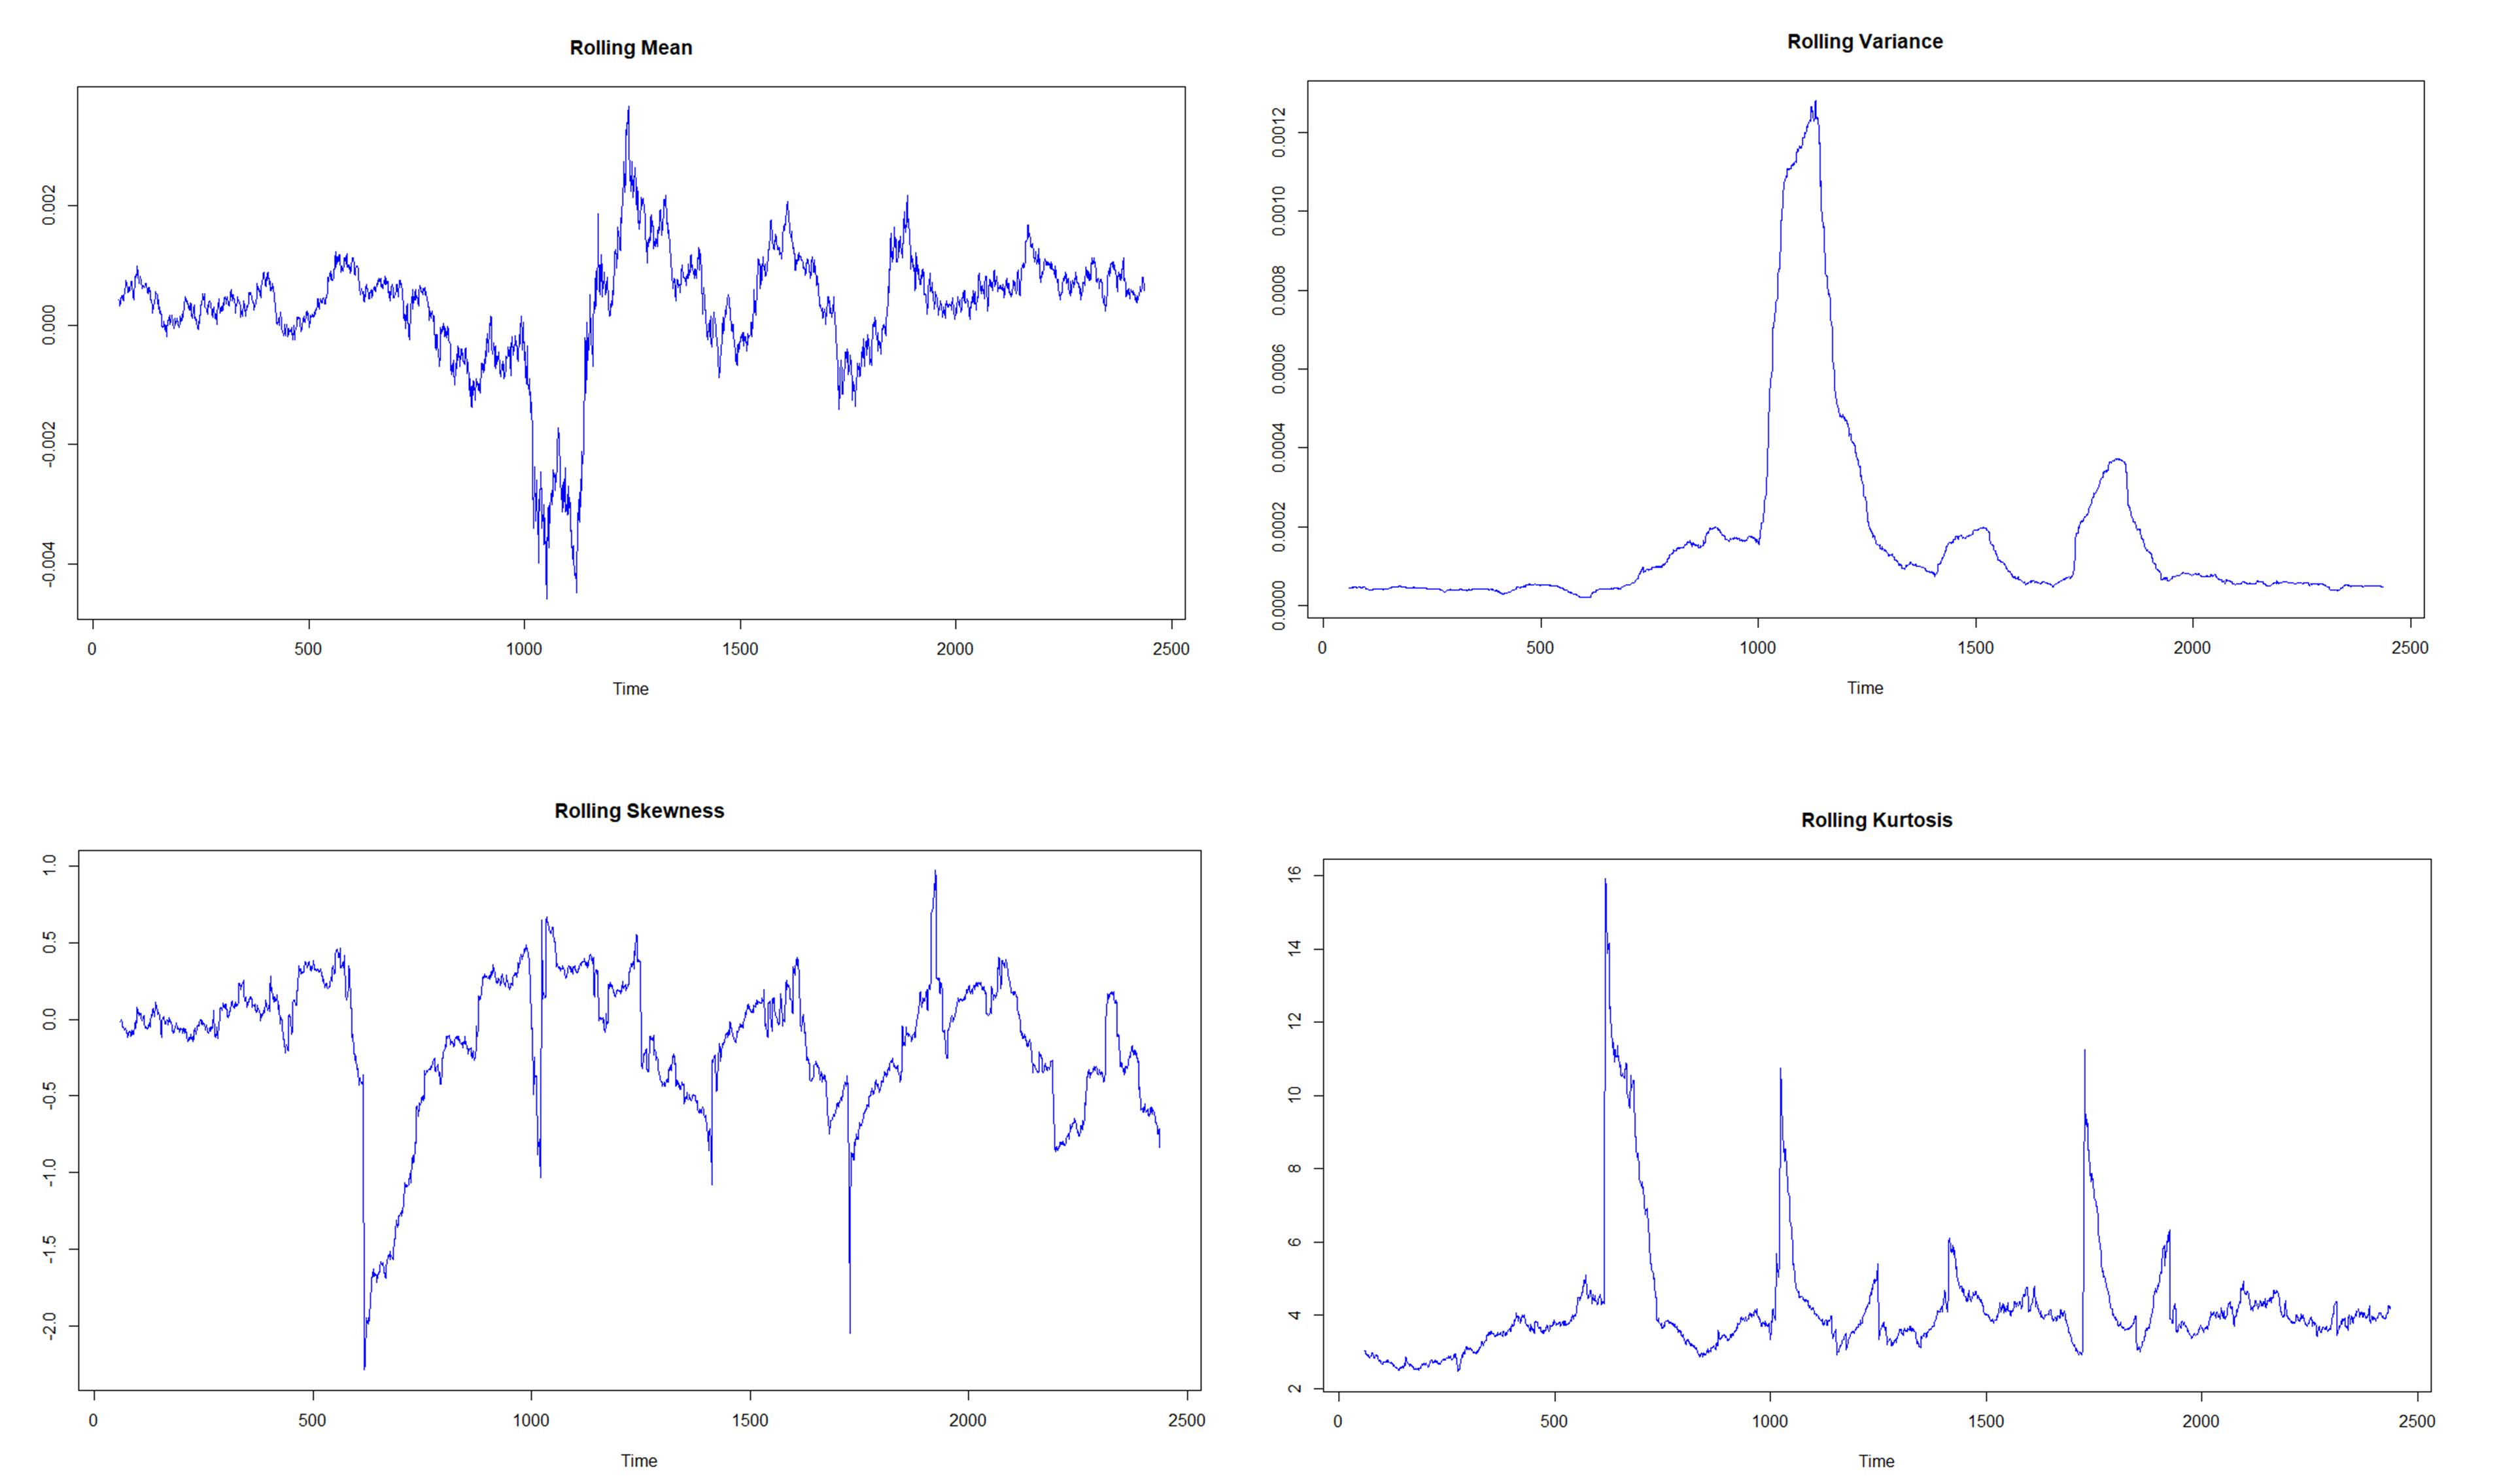
\includegraphics[width=1.05\textwidth]{rolling_return.png}
\caption{\label{fig:roll-ret}Rolling statistics of Return}
\end{figure}

\paragraph{}
The behavior of Rolling mean and variance of RV , as they reach their peaks during the financial crisis, which indicates a high volatility period. The skewness and kurtosis also fluctuate intensively throughout the year, with its extreme peaks cluster in the crisis period.


\begin{figure}[H]
\centering
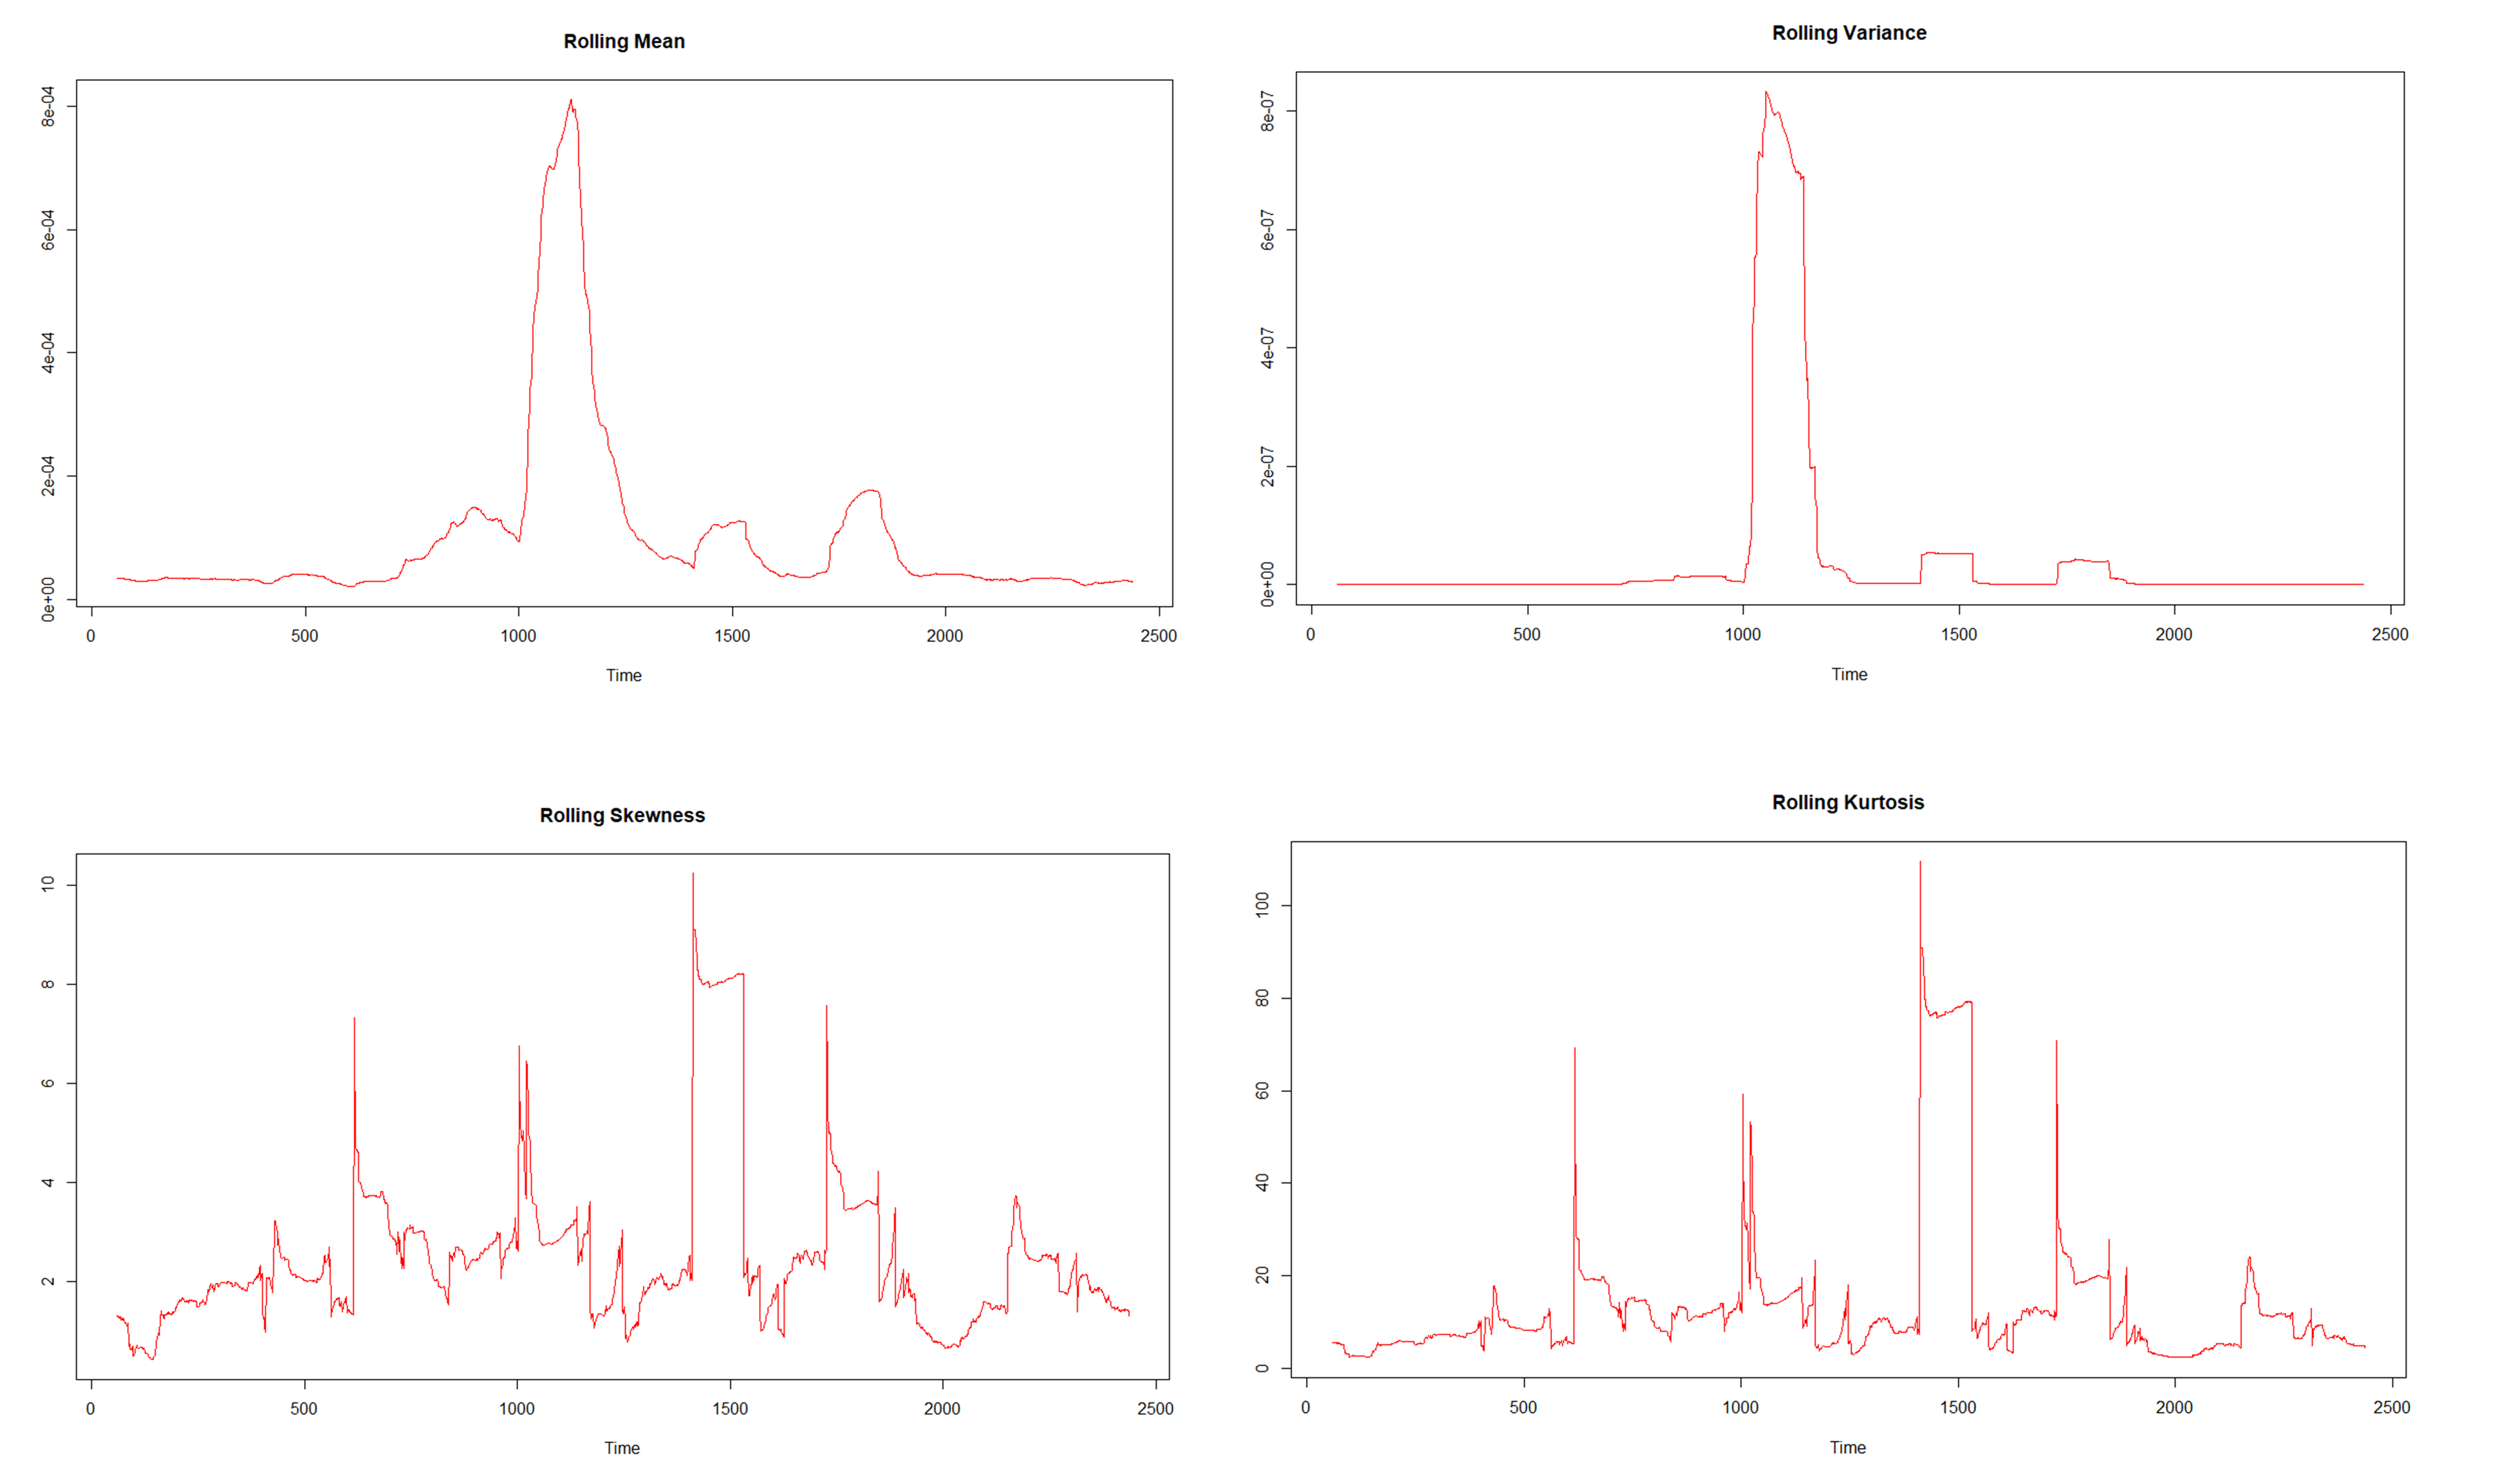
\includegraphics[width=1.05\textwidth]{rolling_rv.png}
\caption{\label{fig:roll-rv}Rolling statistics of RV}
\end{figure}


\section{GARCH Models}

\subsection{Simulation $\mathbf{z_t \sim N(0,1)}$}

\paragraph{}
Consider the \textbf{model 1}, where $z_t i.i.d. D(0,1)$

\begin{eqnarray*}
R_t &=& \mu + \sigma_t z_t \\
\sigma_t^2 &=& \omega + \alpha (R_{t-1} - \theta )^2 + \beta \sigma_{t-1}^2
\end{eqnarray*}

And \textbf{model 2}:

\begin{eqnarray*}
R_t &=& \mu + \sigma_t z_t \\
\sigma_t^2 &=& \omega + \alpha (R_{t-1} - \theta \sigma_{t-1})^2 + \beta \sigma_{t-1}^2
\end{eqnarray*}

With $z_t \sim N(0,1)$, we simulate with the following designs, removing first 250 observations:
\begin{itemize}
\item \textbf{Design 1:} $\Psi = (\mu, \omega, \alpha, \beta, \theta) = (0; 0.01; 0.05; 0.90; 0)$
\item \textbf{Design 2:} $\Psi = (\mu, \omega, \alpha, \beta, \theta) = (0; 0.01; 0.05; 0.60; 2)$
\end{itemize}

With sample size: \textbf{T=100} and \textbf{T=1000}, we estimate $\Psi$ by ML method with \textbf{100 replications}. The results of mean $\Psi$ and std. deviation across the replications is reported in \textbf{Table \ref{tab:sim_norm}}.


%--------- Table: sim_norm --------------%
\begin{table}[H] \centering 
  \caption{Simulation Mean and Std. Deviation of $\Psi$, Normal $z_t$} 
  \label{tab:sim_norm} % for reference 
\begin{tabular}{@{\extracolsep{5pt}}ccccccccc} 
\\[-1.8ex]\hline 
\hline \\[-1.8ex] 
& \multicolumn{4}{c}{\textbf{Model 1}} & \multicolumn{4}{c}{\textbf{Model 2}}\\[-1.8ex]\
& \cline{1-8} 
 & \multicolumn{2}{c}{Design 1} & \multicolumn{2}{c}{Design 2} & \multicolumn{2}{c}{Design 1} & \multicolumn{2}{c}{Design 2}\\
[-1.8ex] & \cline{1-8} 
 & T=100 & T=1000 & T=100  & T=1000  & T=100 & T=1000 & T=100  & T=1000\\ 
\hline \\[-1.8ex] 
mu & \textbf{0.0017} & \textbf{-0.001} & \textbf{0.0028} & \textbf{0.0009} & \textbf{0.0060} & \textbf{0.0017} & \textbf{-0.0212} & \textbf{-0.0023}\\ 
& (0.0433) & (0.0149) & (0.0789) & (0.0212) & (0.0455) & (0.0139) & (0.0818) & (0.0219)\\[1.8ex]

omega & \textbf{0.0242} & \textbf{0.01432} & \textbf{0.0840} & \textbf{0.0304} & \textbf{0.0200} & \textbf{0.0149} & \textbf{0.0818} & \textbf{0.0219}\\
& (0.0332) & (0.0215) & (0.1102) & (0.0435) & (0.0305) & (0.0224) & (0.0678) & (0.0336)\\[1.8ex]

alpha & \textbf{0.0529} & \textbf{0.05116} & \textbf{0.0778} & \textbf{0.0572} & \textbf{0.0440} & \textbf{0.0516} & \textbf{0.0844} & \textbf{0.0572}\\ 
& (0.0769) & (0.0210) & (0.1080) & (0.0220) & (0.0650) & (0.0211) & (0.1080) & (0.0220)\\[1.8ex]

beta & \textbf{0.7727} & \textbf{0.8727} & \textbf{0.6012} & \textbf{0.5685} & \textbf{0.8069} & \textbf{0.8675} & \textbf{0.5892} & \textbf{0.5841}\\ 
& (0.2301) & (0.1199) & (0.3260) & (0.0990) & (0.1923) & (0.1353) & (0.3113) & (0.0929)\\[1.8ex]

theta & \textbf{-0.050} & \textbf{-0.007} & \textbf{0.9707} &\textbf{1.9030} & \textbf{-0.057} & \textbf{0.0480} & \textbf{0.9370} & \textbf{1.778}\\
& (0.7450) & (0.1480) & (0.8640) & (0.4890) & (0.8332) & (0.3346) & (1.054) & (0.5660)\\
\hline \\[-1.8ex] 
\end{tabular} 
\end{table} 
%----------------------------------------------------------------%


For all cases, when the sample size (increase from 100 to 1000), the mean of estimated parameters get closer to the actual ones. Also, with a larger sample, the std. deviation of estimates is smaller. By ML method, we could estimate the actual parameters quite well with a sample size of 1000 in all designs and models.
The comparison of mean and standard deviation of estimates in all designs, sample, model, and distribution of $z_t$ is illustrated in \textbf{Figure \ref{fig:all_sim}.}

\subparagraph*{}
In \textbf{Design 1} $\Psi = (0; 0.01; 0.05; 0.9; 0)$, the estimated results is slightly better than in \textbf{Design 2} $\Psi = (0; 0.01; 0.05; 0.6; 2)$, with smaller standard deviation, and more accurate mean estimates. The standard deviation of estimates is especially worse for $\omega$ in Design 2. Moreover, with small sample size, it is completely fail to estimate to accurate value of $\theta$ that the actual value is not even within +/- 1 SD from the mean of estimates. One explanation could be that in the Design 2  with $\theta \neq 0$, the model is more complicated to estimate. 

The results are not much different in Model 1 and Model 2. The densities of estimated parameters across replications in Design 1 and Design 2 (for Model/Equation 1) is displayed in \textbf{Figure \ref{fig:den_norm}} \footnote{The densities of estimated parameters by Equation 2 could be found in Appendix A.6.}. For small sample size, the variance of estimates is large, though it peaks close to the actual parameters. For design 2, with the small sample size, the estimated results are worse, especially for $\theta$. For large sample size, the estimates has much smaller variance. In all cases, even design 2, we could estimate quite correctly the actual values. The densities peaks at the actual values. The estimated results in Design 2 have slightly larger variance than in Design 1 (for better visualization, see \textbf{Figure \ref{fig:all_sim}}).

\begin{figure}[h]
\centering
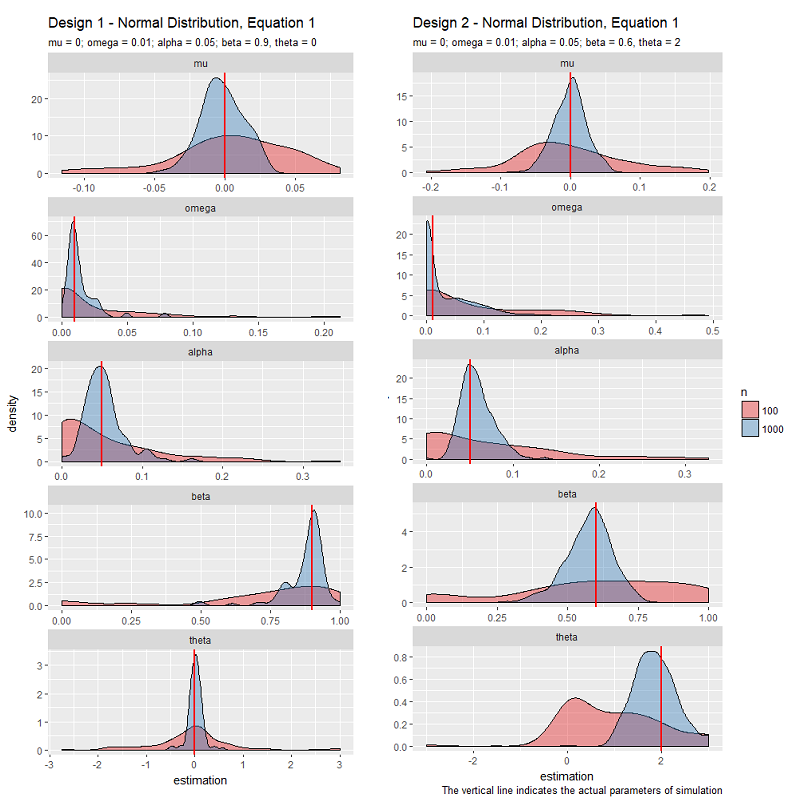
\includegraphics[height=0.5\textheight]{Norm_eq1.png}
\caption{\label{fig:den_norm} Distribution of Estimated Parameters with normal $z_t$}
\end{figure}

\subsection{Simulation $\mathbf{z_t \sim T(10)}$}

\paragraph*{}
We do the same tasks for $z_t \sim T(10)$. That $T(n) = X / \sqrt{Y/n}$, X and Y are independent, $X \sim N(0,1)$ and $Y \sim \chi^2(n)$. The results of mean estimated parameters and std. deviation across the replications is reported in \textbf{Table \ref{tab:sim_std}}. \\

We see the results have same patterns as in the previous part. In larger sample size, the results are more accurate and have smaller std. deviation. The standard deviation of estimates is larger in Design 2. It also fail to estimate the actual $\theta$ in Design 2, for sample with 100 observations. The results are not much different for Model 1 and Model 2. The densities of estimated parameters across replications in Design 1 and 2 (for Model/Equation 1) are in \textbf{Figure \ref{fig:std_den}.}


%--------- Table: sim_std --------------%
\begin{table}[H] \centering 
  \caption{Simulation Mean and Std. Deviation of $\Psi$, Standardized $z_t$} 
  \label{tab:sim_std} % for reference 
\begin{tabular}{@{\extracolsep{5pt}}ccccccccc} 
\\[-1.8ex]\hline 
\hline \\[-1.8ex] 
& \multicolumn{4}{c}{\textbf{Model 1}} & \multicolumn{4}{c}{\textbf{Model 2}}\\[-1.8ex]
& \cline{1-8} 
 & \multicolumn{2}{c}{Design 1} & \multicolumn{2}{c}{Design 2} & \multicolumn{2}{c}{Design 1} & \multicolumn{2}{c}{Design 2}\\
[-1.8ex] & \cline{1-8} 
 & T=100 & T=1000 & T=100  & T=1000  & T=100 & T=1000 & T=100  & T=1000\\ 
\hline \\[-1.8ex] 

mu & \textbf{0.0017} & \textbf{0.0001} & \textbf{-0.0118} & \textbf{-0.0010} & \textbf{0.0057} & \textbf{0.0019} & \textbf{0.0062} & \textbf{0.0050}\\ 
& (0.0550) & (0.0151) & (0.0736) & (0.0260) & (0.0590) & (0.0167) & (0.0859) & (0.0251)\\[1.8ex]

omega & \textbf{0.0605} & \textbf{0.01230} & \textbf{0.1638} & \textbf{0.0394} & \textbf{0.0687} & \textbf{0.0126} & \textbf{0.1621} & \textbf{0.0404}\\ 
& (0.091) & (0.0084) & (0.2050) & (0.0695) & (0.0997) & (0.0107) & (0.2185) & (0.0771)\\[1.8ex]

alpha & \textbf{0.0465} & \textbf{0.0501} & \textbf{0.0700} & \textbf{0.0575} & \textbf{0.0532} & \textbf{0.0530} & \textbf{0.0561} & \textbf{0.0583}\\ 
& (0.0632) & (0.0190) & (0.0854) & (0.0201) & (0.0721) & (0.0211) & (0.0660) & (0.0187)\\[1.8ex]

beta & \textbf{0.6145} & \textbf{0.8840} & \textbf{0.4682} & \textbf{0.5722} & \textbf{0.618} & \textbf{0.8814} & \textbf{0.5050} & \textbf{0.5519}\\ 
& (0.3560) & (0.0490) & (0.3121) & (0.0886) & (0.3550) & (0.0620) & (0.3398) & (0.1218)\\[1.8ex]

theta & \textbf{0.103} & \textbf{0.0230} & \textbf{0.7890} &\textbf{1.803} & \textbf{-0.090} & \textbf{-0.0150} & \textbf{0.7640} & \textbf{1.8420}\\
& (0.8720) & (0.1390) & (0.9303) & (0.5350) & (0.8711) & (0.1437) & (0.9331) & (0.4712)\\
\hline \\[-1.8ex] 
\end{tabular} 
\end{table} 
%----------------------------------------------------------------%



\begin{figure}[h]
\centering
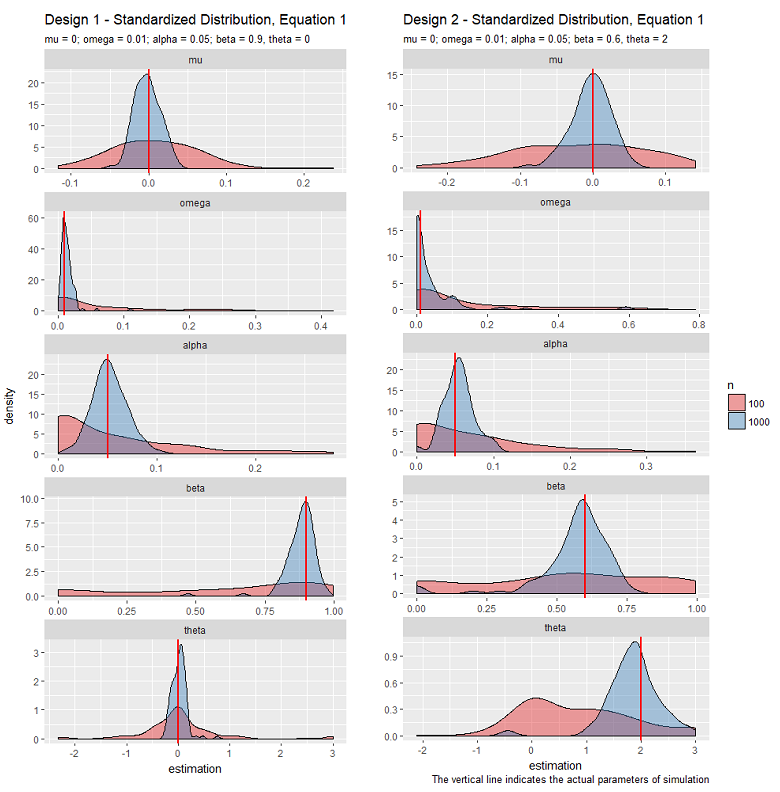
\includegraphics[height=0.5\textheight]{Std_eq1.png}
\caption{\label{fig:std_den} Distribution of Estimated Parameters with standardized $z_t$}
\end{figure}

\subparagraph*{}
Similar to the previous part, when the sample size increases, the variance of estimates decreases, and more peaking at the actual values of parameters. The variance of estimates is slightly larger in Design 2, comparing to Design 1. In general, the estimates are acceptably good in all cases with the sample size of 1000 observations. 

\subparagraph*{}
The mean of estimated parameters and its interval of +/- S.D. is visualized in \textbf{Figure \ref{fig:all_sim}}. Then, we can compare the estimated interval in the cases of normal and standardized distribution. The results are not much different between two cases, but more often, the estimates in normal distribution of $z_t$ generate results with smaller standard deviation. One explanation could be that the $T(10)$ distribution have thicker tail, comparing to the normal distribution. 


\begin{figure}[h]
\centering
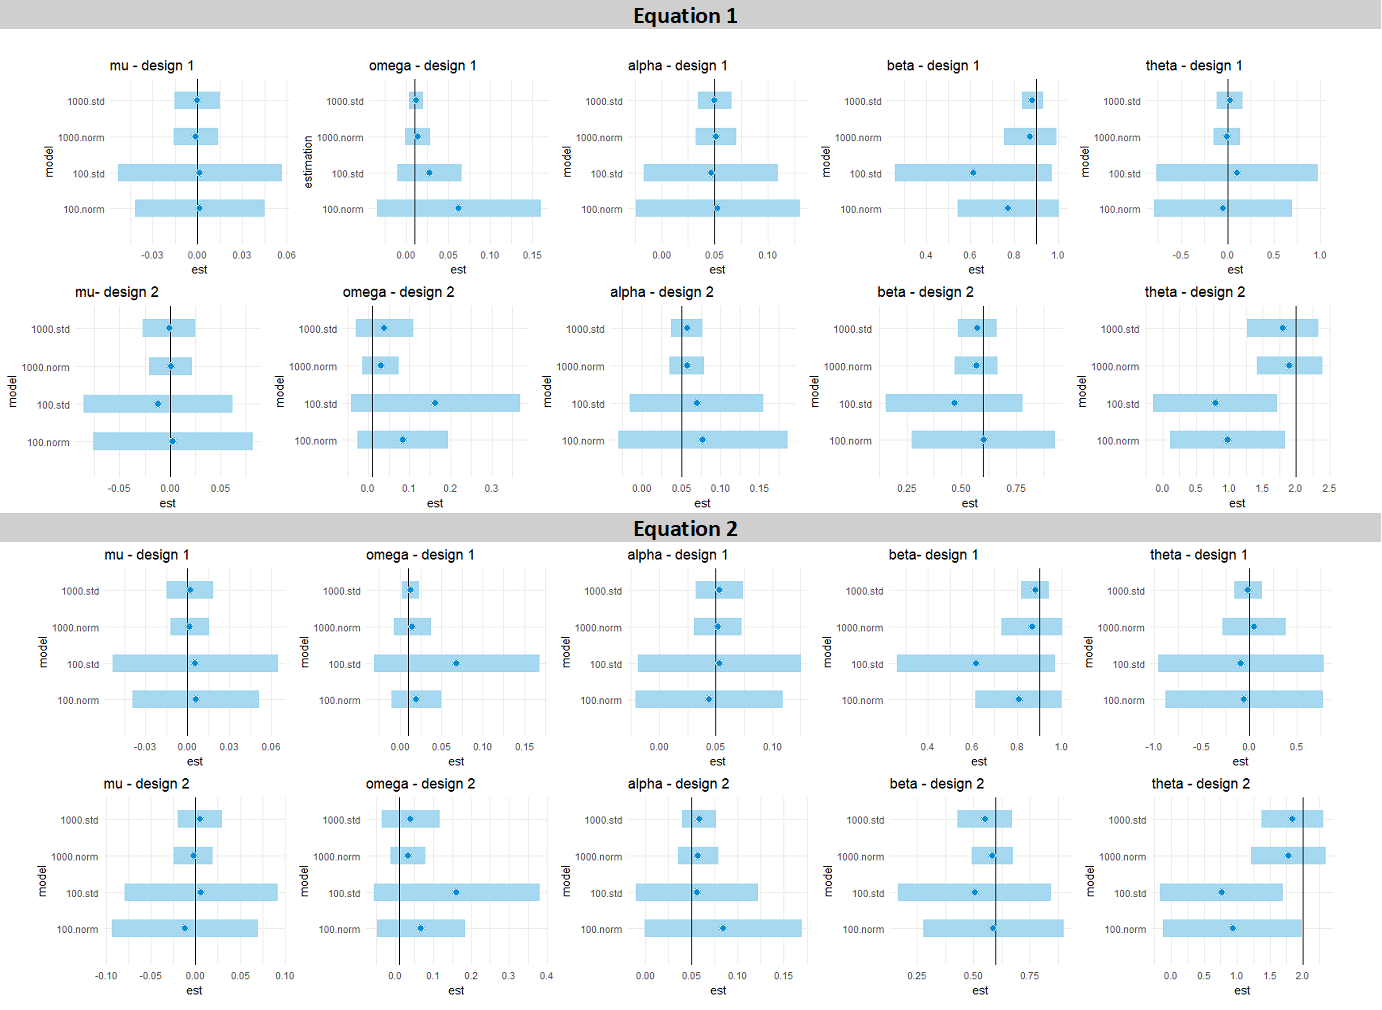
\includegraphics[height=0.45\textheight]{sim_res.png}
\caption{\label{fig:all_sim} Comparing Estimated Parameters in All Simulations}
\end{figure}

\subsection{Estimate GARCH Model}
In \textbf{Section 1}, the ACF plot of the squared observation shows the slow diminishing, which indicates that there is a serial dependence in the variance. These results would motivate us to consider Generalized Autoregressive Conditional Heteroskedasticity (GARCH). \\

In the classical GARCH(p,q) model (without leverage) \cite{bollerslev1986generalized}, $r_t$ is generated by:

\begin{eqnarray}
r_t &=& \mu + \epsilon_t \\
\epsilon &=& z_t h_t^{1/2}\\
h_t &=& \omega + \sum_{i=1}^p \alpha_i \epsilon_{t-i}^2 + \sum^q_{j=1} \beta_j h_{t-j}
\end{eqnarray}

where $\epsilon_t$ denotes a discrete-time stochastic process, $z_t \sim iid(0,1)$, and $h_t = \sigma_t^2$ is the conditional variance at time t. The conditional variance must be strictly positive, so the parameters $\alpha_i$ and $\beta_j$ of the GARCH model must be non-negative. For the stationary, $\sum^p_{i=1} \alpha_i + \sum^q_{j=1} \beta_j < 1$.

\newpage
\paragraph{Model Selection}
\subparagraph{}
To determine the appropriate order of GARCH Model, we use different information criterion Akaike (AIC), Bayes (BIC), Shibata (SIC) and Hannan-Quinn (HQ). The basic idea is that the maximum likelihood of models would be subjects to a penalty for the complexity. All criteria chose the GARCH(2,1) as the best variance model as in \textbf{Table \ref{tab:aic}}. Besides the GARCH for variance model, we use the ARMA(1,1) for the mean model of the returns. This order is also advised preliminarily by ACF and PACF correlogram, and then information criteria. As the baseline, in this part, we choose the generalized distribution model of $z_t$, which is a distribution in exponential family with conditional density is:

\[f(x) = \frac{\kappa e^{ -0.5 |(x - \alpha) / \beta|^{\kappa} }}{2^{1 + \kappa^-1} \beta \Gamma(\kappa^{-1})}\]

The scaled density of $z$, with $\alpha = 0$ and $\beta = \sqrt{2^{-2/\kappa} \frac{\Gamma(3\kappa^{-1})}{\Gamma (3 \kappa^{-1})}} $:
\[f(\frac{x - \mu}{\sigma}) = \frac{1}{\sigma}f(z)\]

with $\alpha, \beta, \kappa$ represent the location, scale and shape parameter. $\kappa$ or \textbf{shape} parameter will be estimated in the model. The smaller values of \textbf{shape}, the flatter density. The normal distribution is the Generalized Error Distribution, with shape = 2 while the Laplace is when the shape = 1. Later, in \textbf{Section 4}, GARCH with normal and student distribution would be implemented.


%--------- Table: Order Selection ----------%

% Change to GARCH ged.

\begin{table}[!htbp] \centering 
  \caption{Model Selection - Information Criterion} 
  \label{tab:aic} % for reference 
\begin{tabular}{@{\extracolsep{5pt}}ccccc} 
\\[-1.8ex]\hline 
\hline \\[-1.8ex] 
 & AIC & BIC & SIC & HQ \\ 
\hline \\[-1.8ex] 
GARCH(1,1) & $-$6.3975 & $-$6.3779 & $-$6.3976 & $-$6.3903 \\ 
GARCH(2,1) & $-$6.4234$^{*}$ & $-$6.4009$^{*}$ & $-$6.4234$^{*}$ & $-$6.4151$^{*}$\\ 
GARCH(1,2) & $-$6.3962 & $-$6.3737 & $-$6.3962 & $-$6.3879\\ 
GARCH(2,2) & $-$6.4200 & $-$6.3898 & $-$6.4200 & $-$6.4100 \\ 
\hline \\[-1.8ex] 
\textit{Note:}  & \multicolumn{4}{r}{$^{*}$ Selected Model, mean model follows ARMA(1,1)} \\ 
\end{tabular} 
\end{table} 

%-----------------------------------------%



\paragraph{Leverage Effects}
\subparagraph*{}
The construction of GARCH (only considering $\epsilon^2_{t-i}$ and $h_{t-i} = \sigma^2_{t-i}$) may fail to explain the asymmetric effect of positive and negative shock $\epsilon_{t-i}$ on volatility $h_t$. It is more realistic to expect the leverage effect in the observed data that negative shock would cause more significant effect to the future volatility than the positive one with the same magnitude. Therefore, the impacts of negative and positive shock should be considered in the model. \\

Three common GARCH-leverage models would be used: EGARCH \cite{nelson1991conditional}, TGARCH \cite{zakoian1994threshold} and APARCH \cite{ding1993long}.

\subparagraph*{}
In \textbf{EGARCH model}, the conditional variance follows the process of natural logarithm:
\[\ln h_t = \omega + \sum^{p}_{i=1} \alpha_i z_{t-i} + \sum^{p}_{i=1} \gamma_i (|z_{t-i}| - E[|z_{t-i}|]) + \sum^q_{j=1} \beta_j \ln h_{t-i}\]
The $z_{t-i}$ is included. In the form of natural logarithm, the non-negative constraint of alpha parameters is not required. The persistence of conditional variance is controlled by parameter $\beta_j$. For the stationary of $\epsilon_t$, it is sufficient that $\beta_j < 1$. Gamma parameters indicates the scale of asymmetric volatility: if $\gamma_i = 0$, there is not asymmetry; if $\gamma_i < 0$, the impacts of negative shock is larger than of positive shocks; if $\gamma_i > 0$, the impacts of positive shock is larger than of negative shocks.

\subparagraph*{}
In \textbf{TGARCH model}, the leverage effect is characterized by the eta parameters:
\[h_t = \omega + \sum^p_{i=1} \alpha_i \epsilon_{t-i}^2 + \sum^p_{i=1} \eta_i S_{t-i} \epsilon_{t-i}^2 +  \sum^q_{j=1} \beta_j h_{t-i}\]

Where $S_{t-i} = 1$ if $\epsilon_{t-i} < 0$, otherwise $S_{t-i} = 0$. Depending on the threshold of zero, $\epsilon_{t-i}^2$ would have different impact on $h_t$. When $\epsilon_{t-i}$ is negative, the impacts of $\epsilon^2_{t-i}$ on $h_t$ is $(\alpha_i + \eta_i)$, where $-1 \leq \eta_i \leq 1$ .If eta parameters are significantly positive, we expect that the negative shocks have larger impact than same magnitude positive shocks.


\subparagraph*{}
In \textbf{APARCH model}, the conditional variance follows:
\[h_t^{\delta / 2} = \omega + \sum^p_{i=1} \alpha_i (|\epsilon_{t-i}| - \gamma_i \epsilon_{t-i})^{\delta} + \sum^{q}_{j=1} \beta_j h_{t-j}^{\delta/2}\]
In which, $\gamma_i$ is the coefficients of leverage terms, while $\delta$ is the asymmetric power parameter: $\delta > 0$ and $-1 \leq \gamma_i \leq 1$. If gamma parameters are significantly positive, the negative shocks have larger impacts. 

To illustrate how different GARCH-leverage models deal with the asymmetric impacts of positive and negative shock $\epsilon_{t-1}$ on conditional volatility $h_t$, we presents the graphs show the relationship between shocks and volatility, estimated by each model in \textbf{Figure \ref{fig:news_curve}}. 

\begin{figure}[h]
\centering
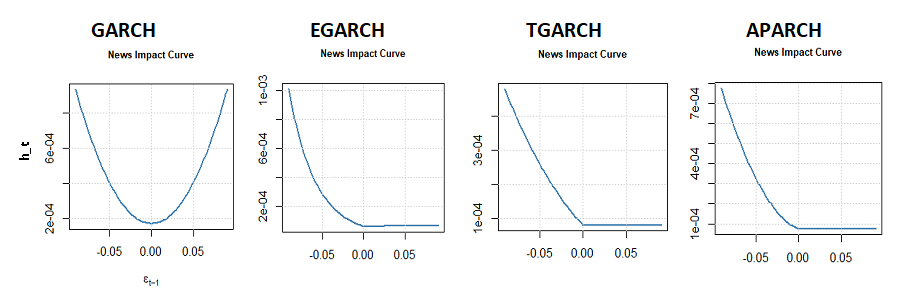
\includegraphics[width=0.6\textheight]{news_impact_curve.png}
\caption{\label{fig:news_curve}Empirical News Impacts Curves of GARCH Models}
\end{figure}

We could see that in GARCH without leverage, the positive and negative $\epsilon_{t-1}$ has symmetric impact (through the zero point), the larger magnitude (far from the zero point) would have higher impacts on $h_t$. Meanwhile, in GARCH versions with leverage: EGARCH, TGARCH, and APARCH, the negative and positive shocks have asymmetric impacts on $h_t$. All estimated news curves from these models shows that the larger negative shocks have larger impacts on $h_t$, while the same magnitude in positive shocks do not have much impact. Yet, different leverage models would have different shapes of curves, which means different weighting for negative shocks.   

\paragraph{Test for the presence of leverage effect}
We adopt the procedure of \cite{engle1993measuring} to detect the asymmetry (leverage effect). 

\begin{itemize}
\item \textbf{Sign bias test:} examine the impact of positive/negative sign of shocks on the conditional variance not predicted by the model, i.e. based on the significant of $b_1$ in the regression: $z_{t} = b_0 + b_1 D_{t-i}^{-} + \nu_t$, where $D_{t-i}^{-} = 1$, if $\epsilon_{t-i}$ is negative, and take 0 otherwise.

\item \textbf{Negative size bias test:} examine if the current model could explain the different effects of different magnitude of negative shocks, based on the significant of $b_2$ in the regression: $z_{t} = b_0 + b_1 D_{t-i}^{-} \epsilon_{t-i} + \nu_t$ 

\item \textbf{Positive size bias test:} examine if the current model could explain the different effects of different magnitude of positive shocks, based on the significant of $b_3$ in the regression: $z_{t} = b_0 + b_3 D_{t-i}^{+} \epsilon_{t-i} + \nu_t$, where $D_{t-i}^{+} = 1$, if $\epsilon_{t-i}$ is positive, and take 0 otherwise.

\item \textbf{Joint Effect:} examine three above simultaneously in the joint model, i.e. testing $H_0: b_1 = b_2 = b_3 = 0$
\end{itemize}

In all cases, the null hypotheses support that there is no remaining leverage effect in the model. The Likelihood ratio test is involved for restricted and unrestricted model. LR test statistic follows the Chi-squared distribution. The results are reported in \textbf{Table \ref{tab:garch}}, in which we reject the null hypothesis that there is no leverage effect in GARCH model.



\paragraph{GARCH Estimation}
\subparagraph*{}
In \textbf{Table \ref{tab:garch}}, we report the estimate of GARCH with and without leverage with the order of model determined by Information Criteria. 500 observations is left as the test set to assess the out-of-sample performance of models.


\subparagraph*{}
In GARCH (2,1) without leverage, all coefficients are significant at 1\%, excepting omega is not significant at 5 \%. In literature, alpha parameters are often interpreted as short-run persistence, while beta parameters signal the long-run persistence. The estimated shape parameter is 1.3559, which is consistent among all models from 1-2C. The estimated distribution of error is not normal (shape = 2). It is closed to Laplace with shape = 1. The empirical standardized residual in comparison to normal distribution and ged(0,1) with estimated shape 1.3559 is in \textbf{Figure \ref{fig:emp_ged_den}}. \\

\begin{figure}[h]
\centering
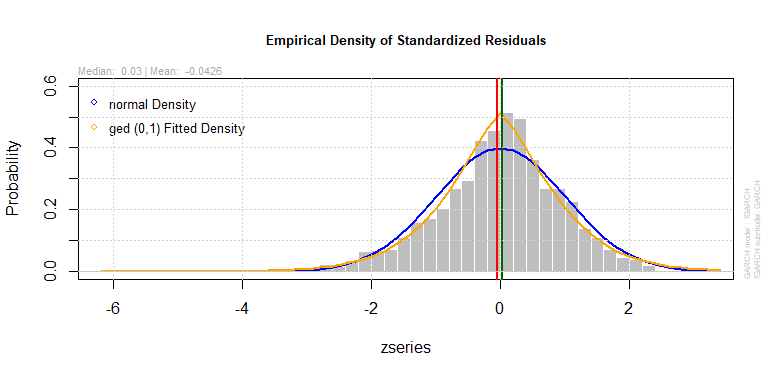
\includegraphics[width=0.5\textheight]{ged_distribution.png}
\caption{\label{fig:emp_ged_den}Empirical Density of Standardized Residuals}
\end{figure}

The parameters indicating leverage effect: $\gamma_i$ and $\eta_i$ are statistically significant in all GARCH models with leverage. The sign of coefficients suggest that the negative shocks will have larger impact than the positive ones with same magnitude (as the previous discussion). 
Confirming that, the asymmetric effect is detected in the test of the presence of leverage effect in GARCH without leverage. We fail to reject the null of sign bias test at 5\%, but this effect is significant at 10\%. The test statistic of negative size bias fails to reject the null of no bias effect. Meanwhile, we reject the null hypothesis in positive size bias at 5\%, and the joint effect is significant at 1\%. 

\subparagraph*{}
EGARCH(2,1) turns to be the best performing leverage model, regarding to Likelihood, IC and the test of remaining leverage effect. It is better than GARCH(2,1) without leverage effect in all of likelihood, AIC, and BIC. This is also the model that there is no remaining asymmetric effect. We fail to reject the null hypotheses in Sign Bias Test, Negative Size Bias, Positive Size Bias, and Joint Effect at all levels. 


%------------ Table: GARCH Ged Estimate -----------------%

\begin{table}[H] \centering 
  \caption{Estimate Results of the GARCH model with Generalized error} 
  \label{tab:garch} 
\begin{tabular}{@{\extracolsep{5pt}} ccccc} 

\\[-1.8ex]\hline 
\hline \\[-1.8ex] 

& & \multicolumn{3}{c}{\textit{GARCH with Leverage Effect}} \\ 
\cline{3-5} 
\\[-1.8ex] & GARCH(2,1) & EGARCH(2,1) & TGARCH(1,1) & APARCH (2,1) 
\\ 
 & (1) & (2) & (2B) & (2C) \\ % Column 1 is OK, we need to fill column 2, 2B, 2C
\hline \\[-1.8ex] 
mu & $0.0005$$^{***}$ &  0.00061$^{***}$ & $0.0005^{***}$ & $0.0005^{***}$ \\
   &$(0.0001)$ & (0.0001) & (0.0001)& (0.0001)\\[1.8ex]

omega & $0.000002$$^{*}$ & $-$0.18107$^{***}$ & $0.0001^{***}$ & $0.000025$  \\ 
&$(0.000001)$& (0.0038)& (0.00005) & (0.0000029)\\[1.8ex]

alpha1 & $0.0408^{***}$ & $-0.25144^{***}$ & $0.0715^{***}$ & $0.0578^{***}$  \\ 
&$(0.0154)$& (0.0428)& (0.0131) & (0.0126)\\[1.8ex]

alpha2 & $0.0419$$^{***}$ & $0.1238^{***}$ & $-$ & $-$ \\
&$(0.0138)$& (0.0418)& & \\[1.8ex]

beta1 & $0.7336$$^{***}$ & $0.9811^{***}$ & $0.9264^{***}$ & $0.9193^{***}$  \\ 
& $(0.0891)$ & $(0.0001)$ & $(0.0136)$ & $(0.0126)$ \\[1.8ex] 

gamma1 & $-$ & $-0.2336^{***}$ & $-$ & $1.0000^{***}$  \\ 
& & (0.0440)& &(0.0005)\\[1.8ex]

gamma2 & $-$ & $0.3844^{***}$ & $-$ & $-$  \\ 
& & (0.0516)& & \\[1.8ex]

eta1 & $-$ & $-$ & $0.9997^{***}$ & $-$  \\ 
& & & (0.1496) & \\[1.8ex]

delta & $-$ & $-$ & $-$ & $1.4102^{***}$  \\ 
& & & & (0.2302)\\[1.8ex]

ar1 & $0.40347$$^{***}$ & $0.4444^{***}$ & $0.3608^{***}$ & $0.5379^{***}$ \\ 
& $(0.0146)$ & (0.0084) & (0.0081) & (0.0470))\\[1.8ex]

ma1 & $-0.4585$$^{***}$ & $-0.5066^{***}$ & $-0.4144^{***}$ & $-0.5897^{***}$  \\ 
& $(0.0170)$ & (0.0093) & (0.0093) & (0.0456)\\[1.8ex]

shape & $1.3559$$^{***}$ & $1.3641^{***}$ & $1.3575^{***}$ & $1.3737^{***}$  \\ 
& $(0.0884)$ & (0.0696) & (0.0709) & (0.0774)\\[1.8ex]

\hline \\[-1.8ex] 
Likelihood & 6421.72 & 6438.47 & 6425.73 & 6427.96\\ 
AIC& -6.4234 & -6.4381 & -6.4274 & -6.4286\\
BIC& -6.4009 & -6.4101 & -6.4049 & -6.4034\\

\hline \\[-1.8ex] 
Sign Bias & 1.735$^{*}$ & 0.2596 & 0.4347 & 0.976\\
Negative Size Bias & 1.109 & 0.0451 & 1.9617$^{**}$ & $2.1421^{**}$\\
Positive Size Bias & 2.489$^{**}$ & 0.3207 & 2.3736$^{**}$ & 2.295$^{**}$\\
Joint Effect & 16.478$^{***}$ & 0.4089 & 9.9938$^{**}$& 11.4711$^{***}$\\
\hline \\[-1.8ex] 

\textit{Note:}  & \multicolumn{4}{r}{$^{*}$p$<$0.1; $^{**}$p$<$0.05; $^{***}$p$<$0.01} \\ 
\end{tabular} 
\end{table} 
%-----------------------------------%

\subparagraph*{}
For TGARCH, the order (1,1) is chosen by IC approach. The sign bias effect turns to be insignificant, while positive size bias and joint effect is less significant than in GARCH without leverage. Yet, the negative size bias effect is significant at 5 \% in this model.
For APARCH, the chosen order is (1,1). Similarly, APARCH can remove the sign bias effect, but the negative size bias becomes significant. Also, the positive size bias and joint effect remain significant. 

\subparagraph*{}
Comparing to conventional GARCH, the models with leverage effect are improved, in terms of likelihood, AIC and BIC. Yet, the remaining leverage effect after TGARCH and APARCH is still significant. These models seems to perform worse in capturing the different effect of large and small negative shocks. EGARCH outperforms, dealing significantly with the leverage effect. We will continue our work with EGARCH as the model with leverage.


\paragraph{In-Sample Diagnostics}
\subparagraph*{}
The series with 2 conditional SD, ACF plots of standardized residuals and squared standardized residuals, Empirical Density and QQ Plot of standardized residuals against theoretical distribution are displayed in \textbf{Figure A.3}. ACF plots of both standardized and squared standardized residuals are well behaved, with most lags lies within the interval. 

\subparagraph*{}
We interest on the distribution and the independence of standardized residuals of GARCH ($\hat{z}_t = \hat{\epsilon}_t / \hat{\sigma}_{t-1})$ with and without leverage. We hope for the standardized residuals to be close to white noise (no serial correlation in residuals and squared residuals), and the distribution is close the assumption of iid. normal distribution. \\

We would conduct the residual diagnostics with:

\begin{itemize}
\item \textbf{Weighted Ljung-Box Test on standardized residuals:} to check any remaining serial correlation in standardized residuals
\item \textbf{Weighted Ljung-Box Test on Squared Stanardized residuals:} to check any remaining serial correlation in standardized squared residuals
\item \textbf{Weighted ARCH LM Test:} to check any remaining ARCH patterns, computed on the auxiliary regression of squared residuals on constant and lagged squared residuals. 
\item \textbf{Adjusted Pearson Gof Test:} Compute the chi-squared gof to compare the empirical distribution of standard residuals with the assumed ones in the model.
\end{itemize}





%------------ Table: In-sample Diagnostics -----------------%

\begin{table}[!htbp] \centering 
  \caption{In-sample Diagnostics} 
  \label{tab:diagnostic} % for reference 
\begin{tabular}{@{\extracolsep{5pt}}ccccccc} 
\\[-1.8ex]\hline 
\hline \\[-1.8ex] 
& \multicolumn{2}{c}{\textit{Generalized}} & \multicolumn{2}{c}{\textit{Normal}} & \multicolumn{2}{c}{\textit{Student}} \\ 
\cline{2-7}
\\[-1.8ex] & GARCH & EGARCH & GARCH & EGARCH & GARCH & EGARCH \\ 
& (1) & (2) & (3) & (4) & (5) & (6) \\ 
\hline \\[-1.8ex] 

& \multicolumn{5}{c}{\textbf{Weighted Ljung-Box Test on Std. Residuals}}\\
\hline \\[-1.8ex] 
Lag [1] & 0.277 & 0.0879 & 0.0280 & 0.1796 & 0.0445 & 0.0175 \\ 
Lag [5] & 2.172 & 1.5692 & 1.6185 & 1.4026 & 1.7724 & 1.5186 \\ 
Lag [9] & 4.446 & 3.8566 & 3.5602 & 3.4142 & 4.0585 & 3.7732 \\  
\hline \\[-1.8ex] 

& \multicolumn{5}{c}{\textbf{Weighted Ljung-Box Test on Std. Squared Residuals}}\\
\hline \\[-1.8ex] 
Lag [1] & 6.369$^{**}$ & 0.0879 & 7.550$^{***}$ & 0.3214 & 5.853$^{**}$ & 0.1703 \\ 
Lag [8] & 7.613 & 1.2115 & 8.848$^{*}$ & 1.4316 & 7.099 & 1.1706\\ 
Lag [14] & 11.578 & 2.5900 & 13.353$^{*}$ & 3.1588 & 10.860 & 2.4551\\
\hline \\[-1.8ex]

& \multicolumn{5}{c}{\textbf{Weighted ARCH LM Tests}}\\
\hline \\[-1.8ex] 
ARCH Lag [4] & 0.097 & 0.0145  & 0.1807 & 0.0528 & 0.0441 & 0.0052 \\ 
ARCH Lag [6] & 0.177 & 0.0195 & 0.3180 & 0.1134 & 0.1316 & 0.0252\\ 
ARCH Lag [8] & 2.486 & 0.2541 & 2.7688 & 0.4120 & 2.4641 & 0.2941\\
\hline \\[-1.8ex] 

& \multicolumn{5}{c}{\textbf{Adjusted Pearson Goodness-of-Fit Test}}\\
\hline \\[-1.8ex] 
Bin 20 & 41.07$^{***}$ & 45.91 $^{***}$ & 80.31$^{***}$ & 76.00$^{***}$ & 43.47$^{***}$ & 53.91$^{***}$ \\ 
Bin 30 & 59.42$^{***}$ & 51.31$^{***}$ & 101.66$^{***}$ & 89.83$^{***}$ & 72.19$^{***}$ & 57.89$^{***}$\\ 
Bin 40 & 74.61$^{***}$ & 62.91$^{***}$ & 111.50$^{***}$ & 94.16$^{***}$ & 79.96$^{***}$ & 73.37$^{***}$\\
Bin 50 & 74.78$^{***}$ & 76.74$^{***}$ & 122.70$^{***}$ & 111.94$^{***}$ & 103.18$^{***}$ & $80.09^{***}$\\
\hline 
\textit{Note:}  & \multicolumn{5}{r}{$^{*}$p$<$0.1; $^{**}$p$<$0.05; $^{***}$p$<$0.01;} \\ 
\end{tabular} 
\end{table} 

%---------------------------------------------%

The diagnostic in-sample results are presented in column (1) and (2), \textbf{Table \ref{tab:diagnostic}}. Both GARCH with and without leverage effect perform acceptably, with no significant remaining serial correlation in residuals and ARCH patterns\footnote{All the lag order chosen for diagnostics test is suggested by the R package 'rugarch'}. \\

While the null of Ljung-Box test on standardized squared residual is reject at 5\% in the GARCH without leverage column (1), it fails to reject the null in the model with leverage column (2). That confirms again the superior of GARCH with leverage in this case, when the presence of leverage effect is detected. 
The difference between empirical distribution of standardized residuals and our assumed distribution ged(0,1) is statistically significant (see: \textbf{Figure A.3}). 

\paragraph*{Out-sample Diagnostic}
\subparagraph*{}
Next, we would evaluate the out-sample performance of models in predicting the volatility. Volatility is unobserved, we use the constructed realized volatility as the proxy for the actual volatility. \\ 

Comparing the model by RMSE (Root Mean Squared error): $RMSE = \sqrt{n^{-1} \sum_{t=1}^{T}(RV_{t} - \hat{\sigma}^2_{t})^2}$ and MAE(Mean Absolute error): $MAE = n^{-1} \sum_{t=1}^{T}|RV_{t} - \hat{\sigma}^2_{t}|$. Other diagnostic of out-sample standardized residuals is also reported in \textbf{Table \ref{tab:diagnostic-out}}. Generalized error in column (1) and (2).\\

The graphs presents the performance of forecasting on out-of-sample is in \textbf{Figure \ref{fig:pred_ged}}, in comparison to actual observed series of daily return. The horizon of 500 observations out-sample is from t = 2000 (2012-06-08) to t = 2500 (2014-06-13). \\

Though in-sample performance of GARCH with leverage is better, GARCH without leverage outperforms in the out-sample, regarding RMSE and MAE. There is no significant serial correlation in standardized and squared standardized, also no remaining ARCH patterns at 5\% in both models. However, the correlation in Lag[1] in GARCH with leverage is weakly significant at 10\%. 

The behavior of standardized residuals, and the diagnostic results are quite different between in-sample and out-sample. One explanation could be that the in-sample set experiences two significant crisis with much larger volatility in those periods, from t=1000 to t=1200 (equivalent to the crisis in 2008 and 2009) and from t=1700 to t=1900 (the crisis in 2011 and 2012), while the observations in out-sample belongs to more "peaceful" and stable period. We might expect that the model with leverage is preferred in the crisis period.\\

\begin{figure}[H]
\centering
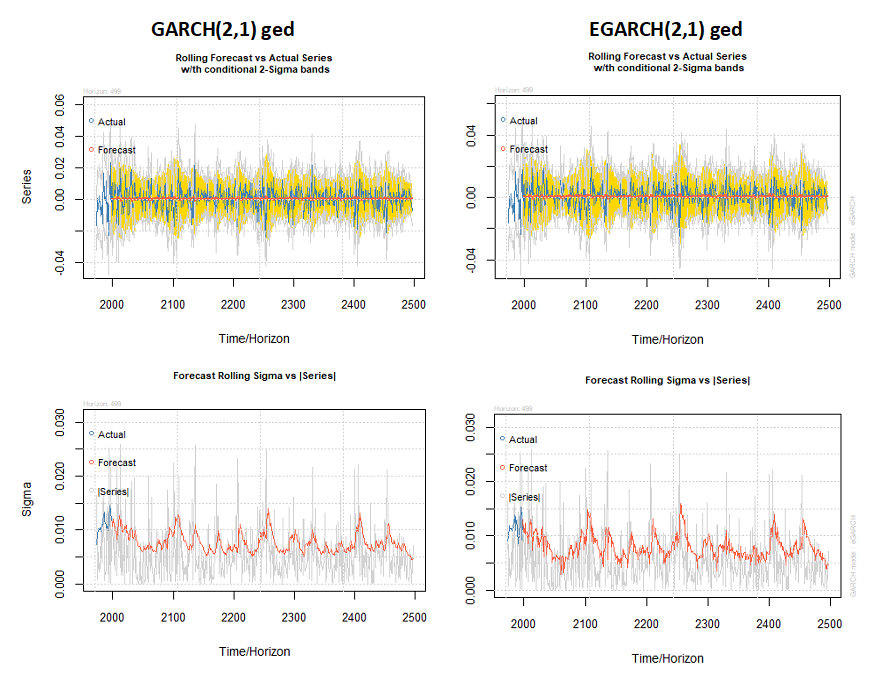
\includegraphics[width=0.8\textwidth]{forecast_ged.png}
\caption{\label{fig:pred_ged}GARCH Generalized Error Model Prediction (Rolling)}
\end{figure}


%-------- Table: Out-sample Diagnostics -----------------%
\begin{table}[H] \centering 
  \caption{Out-sample Diagnostics} 
  \label{tab:diagnostic-out} % for reference 
\begin{tabular}{@{\extracolsep{5pt}}cccccccc} 
\\[-1.8ex]\hline 
\hline \\[-1.8ex] 
 & \multicolumn{2}{c}{\textit{Generalized}} & \multicolumn{2}{c}{\textit{Normal}} & \multicolumn{2}{c}{\textit{Student}} \\ 
\cline{2-7} 
\\[-1.8ex] & GARCH & EGARCH & GARCH & EGARCH & GARCH & EGARCH \\ 
& (1) & (2) & (3) & (4) & (5) & (6) \\ 

\\[-1.8ex]\hline
\\[-1.8ex] RMSE in Vol. & 4.273e-05 & 5.135e-05 & 4.188e-05 & 4.359e-05 & 5.178e-05 & 5.179e-05 \\ 
MAE in Vol. & 3.435e-05 & 3.999e-05 & 3.422e-05 & 4.006e-05 & 3.461e-05 & 4.005e-05\\ 
\hline \\[-1.8ex] 

& \multicolumn{5}{c}{\textbf{Ljung-Box Test on Std. Residuals}}\\
\hline \\[-1.8ex] 
Lag [1] & 0.1150 & 0.4879 & 0.2700 & 1.161 & 0.1989 & 0.5484\\ 
Lag [5] & 7.5941 & 7.5746 & 8.1735 & 8.967 & 7.3857 & 7.0307\\ 
Lag [9] & 13.774 & 13.165 & 14.367 & 14.267& 13.466 & 12.482\\  
\hline \\[-1.8ex] 

& \multicolumn{5}{c}{\textbf{Ljung-Box Test on Std. Squared Residuals}}\\
\hline \\[-1.8ex] 
Lag [1] & 0.1887 & 3.6724$^{*}$ & 0.1002& 3.8431$^{*}$ & 0.1870 & 3.8819$^{**}$\\ 
Lag [8] & 3.5358 & 8.2578 & 3.7374 & 9.4383 & 3.6604 & 8.4611\\ 
Lag [14] & 9.7985 & 16.495 & 10.074 & 17.294 & 9.6773 & 16.558\\
\hline \\[-1.8ex]

& \multicolumn{5}{c}{\textbf{ARCH LM Tests}}\\
\hline \\[-1.8ex] 
ARCH Lag [4] & 1.1198 & 4.3432 & 0.9521 & 4.3963 & 1.2039 & 4.6065\\ 
ARCH Lag [6] & 1.1987 & 5.6379 & 1.1844 & 6.2507 & 1.3220 & 5.8975\\ 
ARCH Lag [8] & 3.5358 & 8.2578 & 3.7374 & 9.4383 & 3.6604 & 8.4611\\

\hline 
\textit{Note:}  & \multicolumn{3}{r}{$^{*}$p$<$0.1; $^{**}$p$<$0.05; $^{***}$p$<$0.01;} \\ 
\end{tabular} 
\end{table} 
%-----------------------------------------%

\subsection{GARCH vs. Riskmetriks vs. Realized Volatility (RV)}
\subparagraph*{}
In this section, we analyze and compare the variance of GARCH model with Riskmetrics filters and Realized Volatility (RV). Consider JP Morgan's RiskMetrics filter as below:
\begin{eqnarray*}
\epsilon_t &=& \sigma_{t-1} u_t \\
\sigma_{t-1}^2 &=& \lambda \sigma_{t-2}^2  + (1 - \lambda) \epsilon_{t-1}^2 = (1 - \lambda) \sum^\infty_{i=1} \lambda^{i-1} \epsilon_{t-i}^2
\end{eqnarray*}

%Compare to a standard GARCH model, where:
%\begin{eqnarray*}
%\sigma_{t-1}^2 &=& \omega + \beta \sigma_{t-2}^2  + \alpha \epsilon_{t-1}^2
%\end{eqnarray*}

RiskMetrics is a special case of GARCH, where the coefficients are constrained as $\omega$ = 0, $\beta$ = $\lambda$ and $\alpha$ = 1 - $\lambda$. Empirically, JP Morgan chose $\lambda$ = 0.94 for daily data. \\
We apply the RiskMetrics filter to the spyder daily return, and obtain the estimation as in \textbf{Table \ref{tab:riskmetrics}}.\\

The differences in terms of coefficients' magnitudes between GARCH, EGARCH and RiskMetrics are trivial. In RiskMetrics, $\omega$ is fixed to be equal 0, and other coefficients are estimated. The value of beta1 (in this case is $\lambda$), equals 0.9273, which is approximate to the JP Morgan's chosen value 0.94. Compare to GARCH and EGARCH, RiskMetrics performance is poorer when considering the Likelihood as well as AIC and BIC. RiskMetrics is not suffered the significant sign bias effect and negative size bias. It means that it deals relatively better with leverage effect, comparing to GARCH. Yet, Positive Size Bias and Joint Effect are both significant in RiskMetrics at 5\%.\\



%------------ Table: GARCH Ged Estimate vs Risk -----------------%

\begin{table}[H] \centering 
  \caption{Estimate Results of the GARCH model with Generalized error and RiskMetrics} 
  \label{tab:riskmetrics} 
\begin{tabular}{@{\extracolsep{4pt}} cccc} 

\\[-1.8ex]\hline 
\hline \\[-1.8ex] 
 
\\[-1.8ex] & GARCH(2,1) & EGARCH(2,1) & RiskMetrics 
\\ 
 & (1) & (2) & (3) \\ % Column 1 is OK, we need to fill column 2, 2B, 2C
\hline \\[-1.8ex] 
mu & $0.0005$$^{***}$ &  0.00061$^{***}$ & $0.0008^{***}$ \\
   &$(0.0001)$ & (0.0001) & (0.0001) \\[1.8ex]

omega & $0.000002$$^{*}$ & $-$0.18107$^{***}$ & $0.0000$ \\ 
&$(0.000001)$& (0.0038)& $-$ \\[1.8ex]

alpha1 & $0.0408^{***}$ & $-0.25144^{***}$ & $0.0726^{***}$  \\ 
&$(0.0154)$& (0.0428)& (0.0100) \\[1.8ex]

alpha2 & $0.0419$$^{***}$ & $0.1238^{***}$ & $-$ \\
&$(0.0138)$& (0.0418)& \\[1.8ex]

beta1 & $0.7336$$^{***}$ & $0.9811^{***}$ & $0.9273^{***}$ \\ 
& $(0.0891)$ & $(0.0001)$ & $-$ \\[1.8ex] 

gamma1 & $-$ & $-0.2336^{***}$ & $-$ \\ 
& & (0.0440)& \\[1.8ex]

gamma2 & $-$ & $0.3844^{***}$ & $-$ \\ 
& & (0.0516)& \\[1.8ex]

ar1 & $0.40347$$^{***}$ & $0.4444^{***}$ & $0.7298^{***}$ \\ 
& $(0.0146)$ & (0.0084) & (0.0500) \\[1.8ex]

ma1 & $-0.4585$$^{***}$ & $-0.5066^{***}$ & $-0.7822^{***}$ \\ 
& $(0.0170)$ & (0.0093) & (0.0449) \\[1.8ex]

shape & $1.3559$$^{***}$ & $1.3641^{***}$ & $1.2845^{***}$ \\ 
& $(0.0884)$ & (0.0696) & (0.0726) \\[1.8ex]

\hline \\[-1.8ex] 
Likelihood & 6421.72 & 6438.47 & 6381.40 \\ 
AIC& -6.4234 & -6.4381 & -6.3860 \\
BIC& -6.4009 & -6.4101 & -6.3720 \\

\hline \\[-1.8ex] 
Sign Bias & 1.735$^{*}$ & 0.2596 & 1.144 \\
Negative Size Bias & 1.109 & 0.0451 & 1.504 \\
Positive Size Bias & 2.489$^{**}$ & 0.3207 & 2.387$^{**}$ \\
Joint Effect & 16.478$^{***}$ & 0.4089 & 11.791$^{***}$ \\
\hline \\[-1.8ex] 

\textit{Note:}  & \multicolumn{3}{r}{$^{*}$p$<$0.1; $^{**}$p$<$0.05; $^{***}$p$<$0.01} \\ 
\end{tabular} 
\end{table} 
%-----------------------------------%


\textbf{In-Sample Diagnostics}\\

We also perform In-sample and Out-of-sample diagnostics for RiskMetrics filter. The results are reported in \textbf{Table \ref{tab:diagnostic-risk}}.

%------------ Table: In-sample Diagnostics -----------------%

\begin{table}[!htbp] \centering 
  \caption{In-sample Diagnostics} 
  \label{tab:diagnostic-risk} % for reference 
\begin{tabular}{@{\extracolsep{4pt}}cccc} 
\\[-1.8ex]\hline 
\hline \\[-1.8ex] 

\\[-1.8ex] & GARCH & EGARCH & RiskMetrics \\ 
& (1) & (2) & (3) \\ 
\hline \\[-1.8ex] 

\multicolumn{4}{c}{\textbf{Weighted Ljung-Box Test on Std. Residuals}}\\
\hline \\[-1.8ex] 
Lag [1] & 0.277 & 0.0879 & 0.2567 \\ 
Lag [5] & 2.172 & 1.5692 & 1.5493 \\ 
Lag [9] & 4.446 & 3.8566 & 3.0555 \\  
\hline \\[-1.8ex] 

\multicolumn{4}{c}{\textbf{Weighted Ljung-Box Test on Std. Squared Residuals}}\\
\hline \\[-1.8ex] 
Lag [1] & 6.369$^{**}$ & 0.0879 & 3.396 \\ 
Lag [2*(p+q)+(p+q)-1] \footnote{Suggested by the R package 'rugarch'} & 7.613 [8] & 1.2115 [8] & 5.488 [5] \\ 
Lag [4*(p+q)+(p+q)-1] & 11.578 [14] & 2.5900 [14] & 6.045 [9] \\
\hline \\[-1.8ex]

\multicolumn{4}{c}{\textbf{Weighted ARCH LM Tests}}\\
\hline \\[-1.8ex] 
ARCH Lag order & 0.097 [4] & 0.0145 [4]  & 0.0314 [3] \\ 
ARCH Lag order & 0.177 [6] & 0.0195 [6] & 0.5221 [5] \\ 
ARCH Lag order & 2.486 [8] & 0.2541 [8] & 0.6607 [7] \\
\hline \\[-1.8ex] 

\multicolumn{4}{c}{\textbf{Adjusted Pearson Goodness-of-Fit Test}}\\
\hline \\[-1.8ex] 
Bin 20 & 41.07$^{***}$ & 45.91 $^{***}$ & 50.82$^{***}$ \\ 
Bin 30 & 59.42$^{***}$ & 51.31$^{***}$ & 59.42$^{***}$ \\ 
Bin 40 & 74.61$^{***}$ & 62.91$^{***}$ & 80.901$^{***}$ \\
Bin 50 & 74.78$^{***}$ & 76.74$^{***}$ & 76.34$^{***}$ \\
\hline 
\multicolumn{4}{c}{\textit{Note: $^{*}$p$<$0.1; $^{**}$p$<$0.05; $^{***}$p$<$0.01; in [ ] are lag-order of tests}} 
\end{tabular} 
\end{table} 

%---------------------------------------------%


The performance of RiskMetrics filter is relatively well, especially compared with the GARCH model without leverage effects (Table 6). At 5\% level, there is no remaining serial correlations exist in both Standard Residuals and Standard Squared Residuals. The null hypothesis for ARCH LM Test is failed to be rejected, and the difference between empirical distribution of standardized residuals and our assumed distribution is statistically significant.\\

\textbf{Out-of-sample Diagnostics}\\

In this step, we perform Out-of-sample performance comparison between GARCH, RiskMetrics and Realized Variance. First, we present a visualization of the prediction of the 3 models in \textbf{Figure \ref{fig:oos_plot} and \ref{fig:boxplot}}.

\begin{figure}[H]
\centering
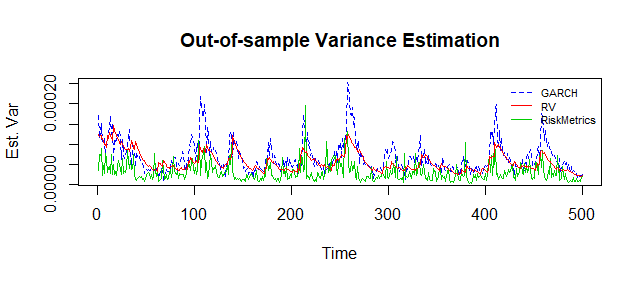
\includegraphics[width=1.05\textwidth]{Rplot01.png}
\caption{\label{fig:oos_plot}Variance Prediction of GARCH, RV and RiskMetrics (Rolling)}
\end{figure}

\begin{figure}[H]
\centering
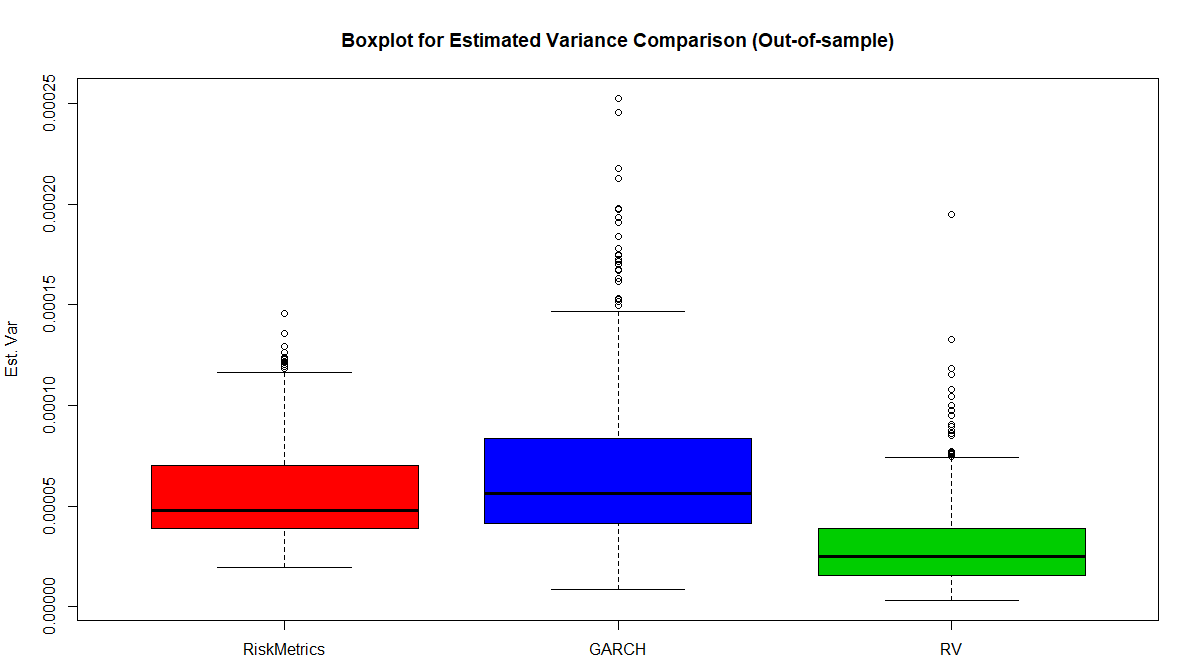
\includegraphics[width=1.03\textwidth]{Rplot02.png}
\caption{\label{fig:boxplot}Variance Prediction of GARCH, RV and RiskMetrics (Rolling)}
\end{figure}

As can be seen from the 2 plots, GARCH model tend to have more extreme predictions with long tail of estimated variance, when it comes to Out-of-sample estimation. It demonstrates an intense volatility, with significantly high peak compared to other predictions. RiskMetrics, on the other hand, provides a relatively "smoother behavior" and more well-capture the Realized Volatility during the stable periods in out-sample set. Thus, by visualization, we can observe that RiskMetrics out-perform the GARCH model when it come to Out-of-sample estimation.\\ 

This result is different from our in-sample interpretations with likelihood, IC, and test of leverage, which preferred EGARCH and GARCH \footnote{We also compare the RiskMetrics with GARCH/EGARCH(1,1), the results are not much different. In fact, GARCH/EGARCH(2,1) outperforms models of (1,1) in out-sample. So, we focus on comparing GARCH/EGARCH(2,1) and RiskMetrics} . But, it is reasonable as the out-sample set includes stable periods (after the crisis in 2008 and 2011), while in-sample set involves periods of crisis. One could expect that the leverage effect become less significant in stable periods, that the EGARCH turns out to be the worst performer in out-sample set. Meanwhile, RiskMetrics with "less-extreme" predicted values outperforms in the stable period (out-sample set). It is not conclusive about the general predicting power of these models. It is possible that EGARCH and GARCH may outperform RiskMetrics if the out-sample set involves some periods of crisis (which is actually not available in this restricted data set).\\

We also conduct Out-of-sample diagnostics for correlation of standardized residuals and remaining ARCH pattern to evaluate the adequacy of models. 
The Out-of-sample diagnostics results in \textbf{Table \ref{tab:diagnostic-out-riskmetrics}} confirm our conclusion. RiskMetrics out-perform both GARCH/EGARCH (2,1) with superior RMSE and MAE. And similar to GARCH and EGARCH, there is no remaining serial correlation of standard residuals and standard squared residuals, as long as ARCH pattern from RiskMetrics filter.

%-------- Table: Out-sample Diagnostics -----------------%
\begin{table}[H] \centering 
  \caption{Out-sample Diagnostics} 
  \label{tab:diagnostic-out-riskmetrics} % for reference 
\begin{tabular}{@{\extracolsep{4pt}}cccc} 
\\[-1.8ex]\hline 
\hline \\[-1.8ex] 
 
\\[-1.8ex] & GARCH & EGARCH & RiskMetrics \\ 
& (1) & (2) & (3)  \\ 

\\[-1.8ex]\hline
\\[-1.8ex] RMSE in Vol. & 4.273e-05 & 5.135e-05 & 3.758e-05 \\ 
MAE in Vol. & 3.435e-05 & 3.999e-05 & 3.031e-05 \\ 
\hline \\[-1.8ex] 

\multicolumn{4}{c}{\textbf{Ljung-Box Test on Std. Residuals}}\\
\hline \\[-1.8ex] 
Lag [1] & 0.1150 & 0.4879 & 0.1519 \\ 
Lag [5] & 7.5941 & 7.5746 & 5.5747 \\ 
Lag [9] & 13.774 & 13.165 & 12.00 \\  
\hline \\[-1.8ex] 

\multicolumn{4}{c}{\textbf{Ljung-Box Test on Std. Squared Residuals}}\\
\hline \\[-1.8ex] 
Lag [1] & 0.1887 & 3.6724$^{*}$ & 0.0679  \\ 
Lag [2*(p+q)+(p+q)-1] & 3.5358 [8] & 8.2578 [8] & 2.8399 [5] \\ 
Lag [4*(p+q)+(p+q)-1] & 9.7985 [14] & 16.495 [14] & 7.8886 [9] \\
\hline \\[-1.8ex]

\multicolumn{4}{c}{\textbf{ARCH LM Tests}}\\
\hline \\[-1.8ex] 
ARCH Lag order & 1.1198 [4] & 4.3432 [4] & 2.2274 [3] \\ 
ARCH Lag order & 1.1987 [6] & 5.6379 [6] & 2.8398 [5] \\ 
ARCH Lag order & 3.5358 [8] & 8.2578 [8] & 3.9404 [7] \\

\hline 
\multicolumn{4}{c}{\textit{Note: $^{*}$p$<$0.1; $^{**}$p$<$0.05; $^{***}$p$<$0.01; in [ ] are lag-order of tests}}
\end{tabular} 
\end{table} 
%-----------------------------------------%



\section{Forecast Compare GARCH and RV}
\subsection{AR(p) model Selection}
\subparagraph{}
To choose the best lag order of AR for the Realized Volatility, we conduct evaluation the Information criterion on a large number of lag. The AIC criterion choose AR(12) as its best model, since AR(12) offers the lowest value of AIC. Regarding BIC criterion, AR(10) is the selected model. Since AR(12) is the chosen model base on AIC, and it also offers second-lowest value of BIC, we decide to adopt lag order 12 for our AR model. In \textbf{Table \ref{tab:aic-rv}}, we present our Model Selection based on Information criterion.


\begin{table}[!htbp] \centering 
  \caption{Model Selection - Information Criterion} 
  \label{tab:aic-rv} % for reference 
\begin{tabular}{@{\extracolsep{3pt}}ccc} 
\\[-1.8ex]\hline 
\hline \\[-1.8ex] 
 & AIC & BIC \\ 
\hline \\[-1.8ex] 
AR(13) & $-$34574.91 & $-$34496.52 \\ 
AR(12) & $-$34576.87$^{*}$ & $-$34504.08 \\ 
AR(11) & $-$34570.46 & $-$34503.27 \\ 
AR(10) & $-$34572.44 & $-$34510.85$^{*}$ \\
AR(9) & $-$34556.54 & $-$34500.54 \\
AR(8) & $-$34351.02 & $-$34300.62 \\
\hline \\[-1.8ex] 
\textit{Note:}  & \multicolumn{2}{r}{$^{*}$ Selected Model} \\ 
\end{tabular} 
\end{table} 

%-----------------------------------------%

\subsection{AR and GARCH comparison}
\subparagraph{}
After fitting the AR(12) to the RV series, period from t=1 ("2004-06-15") to t=1997 ("2012-06-07"), we derive the out-of-sample forecast for the remaining time frame (500 observations).  We also evaluate some errors measurements such as RMSE and MAE, then compare with the forecasting performance of GARCH. Other out-sample diagnostics is also conducted in \textbf{Table \ref{tab:diagnostic-out-ar}}.

%-------- Table: Out-sample Diagnostics -----------------%
\begin{table}[H] \centering 
  \caption{Out-sample Diagnostics} 
  \label{tab:diagnostic-out-ar} % for reference 
\begin{tabular}{@{\extracolsep{4pt}}cccc} 
\\[-1.8ex]\hline 
\hline \\[-1.8ex] 
 
\\[-1.8ex] & GARCH & EGARCH & AR(12) \\ 
& (1) & (2) & (3)  \\ 

\\[-1.8ex]\hline
\\[-1.8ex] RMSE in Vol. & 4.273e-05 & 5.135e-05 & 2.351e-05 \\ 
MAE in Vol. & 3.435e-05 & 3.999e-05 & 1.773e-05 \\ 
\hline \\[-1.8ex]

\multicolumn{4}{c}{\textbf{Ljung-Box Test on Std. Residuals}}\\
\hline \\[-1.8ex] 
Lag [1] & 0.1150 & 0.4879 & 0.0007 \\ 
Lag [5] & 7.5941 & 7.5746 & 2.2315 \\ 
Lag [9] & 13.774 & 13.165 & 6.3557 \\  
\hline \\[-1.8ex] 

\multicolumn{4}{c}{\textbf{Ljung-Box Test on Std. Squared Residuals}}\\
\hline \\[-1.8ex] 
Lag [1] & 0.1887 & 3.6724$^{*}$ & 118.17$^{***}$  \\ 
Lag [8 & 3.5358 & 8.2578 & 291.32$^{***}$ \\ 
Lag [14] & 9.7985 & 16.495 & 473.73$^{***}$ \\
\hline \\[-1.8ex]

\multicolumn{4}{c}{\textbf{ARCH LM Tests}}\\
\hline \\[-1.8ex] 
ARCH Lag [4] & 1.1198 & 4.3432 & 248.7113$^{***}$ \\ 
ARCH Lag [6] & 1.1987 & 5.6379 & 274.931$^{***}$ \\ 
ARCH Lag [8] & 3.5358 & 8.2578 & 291.3208$^{***}$ \\

\hline 
\end{tabular} 
\end{table} 
%-----------------------------------------%

As can be seen, AR(12) demonstrate superior performance in out-of-sample forecasting compare to GARCH and GARCH with leverage effect model. Both RMSE and MAE of GARCH and EGARCH is significantly higher than of AR(12) model. However, on the out-of-sample diagnostics, AR(12) reveals its downsides. While serial correlation could not be found in Standard Residuals, it does have significant existence in Squared Residuals. ARCH pattern is also found in the Residuals of AR(12). In conclusion, the Residuals itself is non-autocorrelated but its squared transformation is, and ARCH pattern still exist. 
A visualization of out-of-sample forecasting from AR(12) model is represented below:

\begin{figure}[H]
\centering
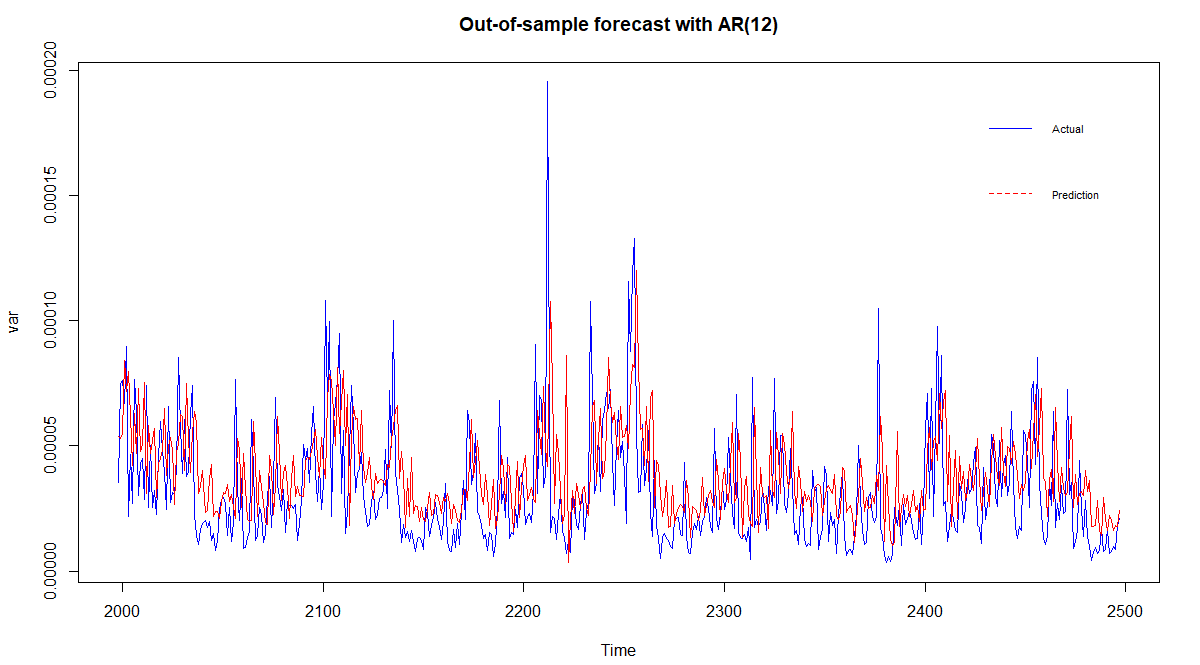
\includegraphics[width=1.05\textwidth]{AR12.png}
\caption{\label{fig:ar12}Rolling Out-of-sample forecast of AR(12) model}
\end{figure}




\section{Value-at-Risk}

\subsection{GARCH Normal and Student Error}

\subparagraph*{}
We apply the GARCH with and without model in normal and student error. The student distribution is described by the \textbf{shape} parameter (degree of freedom), which is also estimated and reported in the table. The results are reported in \textbf{Table \ref{tab:student}}, column (3)-(6). 
The diagnostics in-sample is in \textbf{Table \ref{tab:diagnostic}}, and out-sample diagnostics in \textbf{Table \ref{tab:diagnostic-out}}, column (3)-(6). \\



%-------- Table Normal - Std GARCH ---------%

\begin{table}[H] \centering 
  \caption{Estimate Results of the GARCH model with Normal and Student Error} 
  \label{tab:student} 
\begin{tabular}{@{\extracolsep{5pt}} ccccccc} 

\\[-1.8ex]\hline 
\hline \\[-1.8ex] 

& \multicolumn{2}{c}{\textit{Generalized}} & \multicolumn{2}{c}{\textit{Normal}} & \multicolumn{2}{c}{\textit{Student}}\\ 
\cline{2-7} 
\\[-1.8ex] & GARCH & EGARCH & GARCH & EGARCH & GARCH & EGARCH 
\\ 
& (1) & (2) & (3) & (4) & (5) & (6) \\ 
\hline \\[-1.8ex] 
mu & 0.0005$^{***}$ & 0.00061$^{***}$ & $0.0001$ & $0.0002$ & $0.0005^{***}$ & $0.0006^{***}$ \\
   & (0.0001) & (0.0001) & $(0.0001)$ & (0.0001) & (0.0001) & (0.0001)\\[1.8ex]

omega & 0.000002$^{*}$ & $-0.18107^{***}$ & $0.000003^{***}$ & $-$0.2169$^{***}$ & $0.000002$ & $-0.1491^{***}$  \\ 
& (0.000001) & (0.0038) &$(0.000001)$& (0.0034)& (0.000001) & (0.0038)\\[1.8ex]

alpha1 & 0.0408$^{***}$ & $-0.2514^{***}$ & $0.0382$$^{***}$ & $-0.2206^{***}$ & $0.0409^{***}$ & $-0.2645^{***}$  \\ 
& (0.0154) & (0.0428) &$(0.0035)$& (0.0141)& (0.0145) & (0.0431)\\[1.8ex]

alpha2 & 0.0419$^{***}$ & 0.1238$^{***}$ & $0.0404$$^{***}$ & $0.0964^{***}$ & $0.0437^{***}$ & $0.1368^{***}$ \\
& (0.0138) & (0.0418) &$(0.0023)$& (0.0088)& (0.0069)& (0.043)\\[1.8ex]

beta1 & 0.7336$^{***}$ & 0.9811$^{***}$ & $0.7430$$^{***}$ & $0.9759^{***}$ & $0.7298^{***}$ & $0.9843^{***}$  \\ 
& (0.0891) & (0.0001) & $(0.0159)$ & $(0.0001)$ & $(0.0383)$ & $(0.000022)$ \\[1.8ex] 

gamma1 & $-$ & $-0.2336^{***}$ & $-$ & $-0.2128^{***}$ & $-$ & $-0.2396^{***}$  \\ 
& & & & (0.0476)& &(0.0405)\\[1.8ex]

gamma2 & $-$ & 0.3844$^{***}$& $-$ & $0.3625^{***}$ & $-$ & $0.3889^{***}$  \\ 
& & (0.0516) & & (0.0476)& & (0.0507)\\[1.8ex]

shape & 1.3559$^{***}$ & 1.3641$^{***}$& $-$ & $-$ & $6.9301^{***}$ & $6.7449^{***}$  \\ 
& (0.0884) & (0.0696) & & & (2.0112) & (1.1151)\\[1.8ex]

ar1 & $0.4035^{***}$ & $0.4444^{***}$ & $0.2899$ & $0.3250^{***}$ & $0.4175$ & $0.5086^{***}$ \\ 
& (0.0170) & (0.0093) & $(0.2649)$ & (0.0229) & (0.2749) & (0.0137))\\[1.8ex]

ma1 & $-0.4585^{***}$ & $-0.5066^{***}$ & $-0.3540$ $^{***}$ & $-0.3994^{***}$ & $-0.4796^{*}$ & $-0.5732^{***}$  \\ 
& (0.0170) & (0.0093) & $(0.2594)$ & (0.0230) & (0.2543) & (0.0137)\\[1.8ex]

\hline \\[-1.8ex] 
Likelihood & 6421.72 & 6438.47 & 6386.735 & 6403.48 & 6417.89& 6437.958\\ 
AIC & -6.4234 & -6.4381 & -6.3893 & -6.4041 & -6.4195 &-6.4376\\
BIC & -6.4009 & -6.4101 & -6.3697 & -6.3789 & -6.3971 & -6.4096\\
\hline \\[-1.8ex] 
Sign Bias & 1.735$^{*}$ & 0.2596 & 2.028$^{**}$ & 0.008 & 1.548 & 0.4064\\
Negative Size & 1.109 & 0.0451 & 1.081 & 0.341 & 1.223 & 0.3606\\
Positive Size & 2.489$^{**}$ & 0.3207 & 2.387$^{**}$ & 2.690$^{***}$ & 1.9621$^{**}$ & 0.0419\\
Joint Effect & 16.478$^{***}$ & 0.4089 & 17.796$^{***}$ & 0.359 & 16.672$^{***}$& 0.7359\\
\hline \\[-1.8ex] 
\textit{Note:}  & \multicolumn{3}{r}{$^{*}$p$<$0.1; $^{**}$p$<$0.05; $^{***}$p$<$0.01} \\ 
\end{tabular} 
\end{table} 
%---------------------------------------------------%

The series with 2 conditional SD, ACF plots of standardized residuals and squared standardized residuals, Empirical Density and QQ Plot of standardized residuals versus theoretical distribution are displayed in \textbf{Figure A.1} and \textbf{Figure A.2}. ACF plots of both standardized and squared standardized residuals are well behaved, with most lags lies within the interval.\\

Regarding to AIC and BIC, models with generalized error are preferred to the ones with normal and student error. The student error models are better than the ones with normal error. Nevertheless, the estimates of parameters in all models are not much different in magnitude, sign and significance. 
The test detects always detect the leverage effect in all models without leverage. In most the cases (excepting normal error model in positive size bias), the EGARCH is quite successful to deal with leverage effect, not rejecting any null hypotheses of no bias effect at any level. \\

For the diagnostics in-sample \textbf{Table \ref{tab:diagnostic}}, the GARCH without leverage in normal and student error is subject to the serial correlation in squared residuals. Yet, the standardized residual are well-behaved in the version with leverage, all null hypotheses are not rejected. \\

In out-sample, the pattern is similar to the GARCH with generalized error. While the leverage-model outperforms in in-sample set, it is worse than the model without leverage in out-sample set. Among all three distribution model of error, the normal models have the best RMSE and MAE, while the GARCH with student seems to be the least favorable. It is also different from the in-sample interpretation that generalized error model is the most adequate, and the student error model is slightly preferred to the normal error. The graphs of forecast by normal and student error models is illustrated in comparison to actual observations in \textbf{Figure A.4}. 


\subsection{VaR 5\% Violation Sample and Tests}

\subparagraph*{}
For each model on the training and test sample, we compute the $VaR^{(0.05)}$. In \textbf{Table \ref{tab:var} }, we report the violation rate, $\frac{\mathbf{1}\left[R_t \leq VaR_t^{(\alpha)}\right]}{T}$, and the results of three tests on the behavior of $H_t$:
\[P(H_t = 1) = P(R_t \leq VaR_t^{(0.05)} | I_{t-1})\]

In term of violation ratio, Normal models outperform in both training and test set. Between leverage and no-leverage model, the out-sample rate is quite the same. The cluster of $VaR$ Violations (in magnitude) by models is illustrated in \textbf{Figure A.5}. For more interesting results, we also report and compare the VaR violation of Riskmetrics model. \\

To check the correctly specified models, we conduct three tests on the sample of VaR violation.

\paragraph{Test 1: Unconditional Distribution of $\mathbf{H_t}$ is Bernoulli$\mathbf{(\alpha)}$} 

With the $T_0$ and $T_1$ are the numbers of $H_t$ zeros and ones in the sample, the likelihood:

\[L(p) = \prod^{T}_{t=1}(1-\pi)^{1-H_t} \pi^{H_t} = (1-\pi)^{T_0} \pi^{T_1}\]

The unconditional MLE estimator of $\pi$ is: $\hat{\pi} = T_1 / T$. The log-likelihood ratio test under the null is:

\[LR_{uc} = 2[log(L(\hat{\pi})) - log(L(\alpha))] \sim \chi^2(1)\]

\subparagraph*{}
\textbf{Results:} For in-sample, the null is rejected in all models. The normal models are slightly better when the null is only rejected at 5\% and 10\% for the with and without leverage model, respectively. For out-sample, the test fails to reject the null of unconditional Bernoulli$(\alpha)$ in all models.



\paragraph{Test 2: $\mathbf{H_t}$ is i.i.d. and Bernoulli $\mathbf{(\alpha)}$}

In this part, we want to test the i.i.d of $H_t$ against a simple alternative that the it follows a homogeneous Markov Chain:

\[\Pi = \begin{bmatrix}
    1 - \pi_{01} & \pi_{01}\\
    1 - \pi_{11} & \pi_{11}
  \end{bmatrix}\]
  
where: $\pi_{11} = P[H_t=1 | H_{t-1}=1]$ and $\pi_{01} = P[H_t = 1 | H_{t-1} = 0]$. \\

The Likelihood of the Markov Chain is:
\[L(\Pi) = (1-\pi_{01})^{T_{00}} \pi_{01}^{T_{01}} (1-\pi_{11})^{T_{10}} \pi_{11}^{T_{11}}\]

The MLE estimator of $\pi_{01}$ and $\pi_{11}$ are:
\[\hat{\pi}_{01} = \frac{T_{01}}{T_{00}+T_{01}}, \hat{\pi}_{11} = \frac{T_{11}}{T_{10} + T_{11}}\]

while $\hat{\pi}_{00} = 1 - \hat{\pi}_{01}$, $\hat{\pi}_{10} = 1 - \hat{\pi}_{11}$.

The log-likelihood ratio test under the null is: 

\[LR_{cc} = 2[\log L(\hat{\Pi}) - \log L(\alpha)] = LR_{uc} + LR_{ind} \sim \chi^2(2) \]

\subparagraph*{}
\textbf{Results:} For in-sample, the null is rejected in most of models, excepting GARCH normal error without leverage and the null in the normal error model with leverage is only rejected at 10\%. Once again, the normal models relatively outperform. For out-sample, the test fails to reject the null in all models. 

\paragraph{Test 3: Add explanatory variable to explain $\mathbf{H_t}$}

From the given dataset, we use $BV_{t-1}$ and $RJ_{t-1}$ as explanatory variable for $H_t$:
\[H_t = b_0 + b_{BV,t-1} BV_{t-1} + b_{RJ,t-1} RJ_{t-1} + e_{t}\]
We will expect that in the appropriate model: $E[H_t | I_{t-1}] = \alpha$ and $Cov[H_t, x_{t-1}] = 0, \forall x_{t-1} \in I_{t-1}$, hence $b_0 = \alpha$; $b_{BV,t-1} = 0$, and $b_{RJ,t-1} = 0$. \\

\textbf{Results:} In-Sample, the effect of $BV_{t-1}$ on $H_t$ is significant in EGARCH-ged at 5\%, Riskmetrics at 5\%. EGARCH-norm and EGARCH-student at 1\% and 5\%, respectively. However, this effect is no more significant in all models for out-sample set. The effect of $RJ_{t-1}$ as explanatory variable is not significant in all models for both in-sample and out-sample. The null hypothesis that $b_0 = \alpha$ is not reject in most of models for in-sample set, excepting the EGARCH-student and Riskmetrics have the null rejected at 5\% and 1\% respectively. \\

\paragraph{Further comments}
Regarding Value-at-Risk, the normal models GARCH outperforms among 6 models. Out-of-sample, it always fails to reject the null hypotheses that the model is correctly defined: $H_t$ is Bernoulli$(\mathbf{\alpha})$ and i.i.d.; $E[H_t | I_{t-1}] = \alpha$ and $Cov[H_t, x_{t-1}] = 0, \forall x_{t-1} \in I_{t-1}$. The in-sample performance of normal models is acceptable when most of null hypotheses is not rejected at 1\%. The models with student error have the null of tests rejected in in-sample set at 1\%, but not rejected at any level out-of-sample. \\

For the Riskmetrics model, it has the least favourable results in tests of VaR violation, comparing to all other models. It is reasonable, as the previous explanation in \textbf{Section 2.4}, RiskMetrics predicts lower values (less extreme) of volatility comparing to GARCH. \\

One can see that the violation rate and the behavior of VaR violation in out-sample set is much more well-behaved, comparing to the results in in-sample set. One explanation could be that the in-sample set experiences two significant crisis with much larger volatility (and also VaR violation) in those periods, from t=1000 to t=1200 (equivalent to the crisis in 2008 and 2009) and from t=1700 to t=1900 (the crisis in 2011 and 2012), while the observations in out-sample belongs to more "peaceful" and stable period.\\

Even though the models with leverage has better results in in-sample diagnostics, its performance out-of-sample is not better or even worse, in terms of VaR violations. For in-sample set, the models with generalized error and leverage effects have more preferred results in likelihood, IC and diagnostic tests. But, in out-of-sample, the models with normal error and without leverage effects have more preferred results in diagnostic tests, RMSE and VaR violation rate.   

%--------- Table VaR -------------------------%
\begin{table}[H] \centering 
  \caption{VaR 5\% Violation Sample and Tests} 
  \label{tab:var} % for reference 
\begin{tabular}{@{\extracolsep{5pt}}cccccccc} 
\\[-1.8ex]\hline 
\hline \\[-1.8ex] 
& \multicolumn{2}{c}{\textit{Generalized}} & \multicolumn{2}{c}{\textit{Normal}} & \multicolumn{2}{c}{\textit{Student}} \\ 
\cline{2-7}
\\[-1.8ex] & GARCH & EGARCH & GARCH & EGARCH & GARCH & EGARCH & RMetrics \\ 
 & (1) & (2) & (3) & (4) & (5) & (6) & (7) \\ 
\hline \\[-1.8ex] 
\multicolumn{3}{l}{\textbf{Violation Rate }}& \\[1.8ex]
In-sample & 0.0625 & 0.0651 & 0.0590 & 0.0615 & 0.0640 & 0.0696 & 0.0676 \\ 
Out-sample & 0.0520 & 0.0500 & 0.0460 & 0.0460 & 0.0580 & 0.0540 & 0.0620 \\ [1.8ex]
\hline \\[-1.8ex] 

&\multicolumn{7}{c}{\textbf{Null: Unconditional distribution of $\mathbf{H(t)}$ is Bernoulli($\mathbf{\alpha}$)}} \\
\hline \\[-1.8ex]
% check the p-val to put star (df=1), via http://www.socscistatistics.com/pvalues/chidistribution.aspx
In-sample & 6.1960$^{**}$ & 8.786$^{***}$ & 3.2899$^{*}$ & 5.2784$^{**}$ & 7.7002$^{***}$ & 14.477$^{***}$ & 11.789$^{***}$\\ 
Out-sample & $0.0415$ & 0.0158 & 0.1728 & 0.1728 & 0.6421 & 0.6421 & 1.4130  \\ [1.8ex]
\hline \\[-1.8ex]

&\multicolumn{7}{c}{\textbf{Null: $\mathbf{H(t)}$ is i.i.d and Bernoulli($\mathbf{\alpha}$)}} \\
\hline \\[-1.8ex] 
% chi-squa. df = 2
In-sample & 6.3257$^{**}$ & 8.849$^{**}$ & 3.4702 & 5.3291$^{*}$ & 7.7363$^{**}$ & 14.531$^{***}$ & 11.919$^{***}$\\ 
Out-sample & $0.1586$ & 2.6384 & 0.1684 & 2.3881 & 1.0211 & 0.0347 & 2.0398\\ [1.8ex]
\hline \\[-1.8ex]

&\multicolumn{7}{c}{\textbf{Add explanatory to explain the violation}} \\
\hline \\[-1.8ex] 
\multicolumn{3}{l}{$\mathbf{H_0: b_0 = \alpha}$} & \\
In-Sample & 1.3419 & 1.549 & 0.964 & 0.973 & 1.7310$^{*}$ & 2.284$^{**}$ & 2.333$^{***}$\\ 
Out-sample & $-0.7953$ & $-0.5451$ & $-0.014$ & $-0.4909$ & $-0.1224$ & 1.4530 & $-0.3011$\\ [1.8ex]

\multicolumn{3}{l}{$\mathbf{H_0: b_{BV,t-1}= 0}$} & \\
In-Sample & 1.4511 & 2.3985$^{**}$ & 1.6443 & 2.787$^{***}$ & 1.3338 & 2.094$^{**}$ & 1.964$^{**}$\\ 
Out-Sample & $0.6214$ & $0.3065$ & $0.9606$ & $-0.1436$ & $0.3789$ & $0.2131$ & 1.0436 \\ [1.8ex]

\multicolumn{3}{l}{$\mathbf{H_0: b_{RJ,t-1}= 0}$} & \\
In-Sample & 0.1219 & $-0.264$ & $-0.2334$ & $-0.292$ & $-0.2043$ & $-0.412$ & $-0.961$\\ 
Out-Sample & $1.3695$ & $0.9960$ & $0.9675$ & $0.5169$ & $0.7700$ & $0.6482$ & 0.4548 \\ 
\hline 
\\[-1.8ex]
\textit{Note:}  & \multicolumn{6}{r}{$^{*}$p$<$0.1; $^{**}$p$<$0.05; $^{***}$p$<$0.01; table reports the test values} \\ 
\end{tabular} 
\end{table} 
%----------------------------------------------------------%




\bibliographystyle{apalike}
\bibliography{sample}

%----------------------------------------------------%
% APPENDIX

% A1. Norm fit (10 graphs)
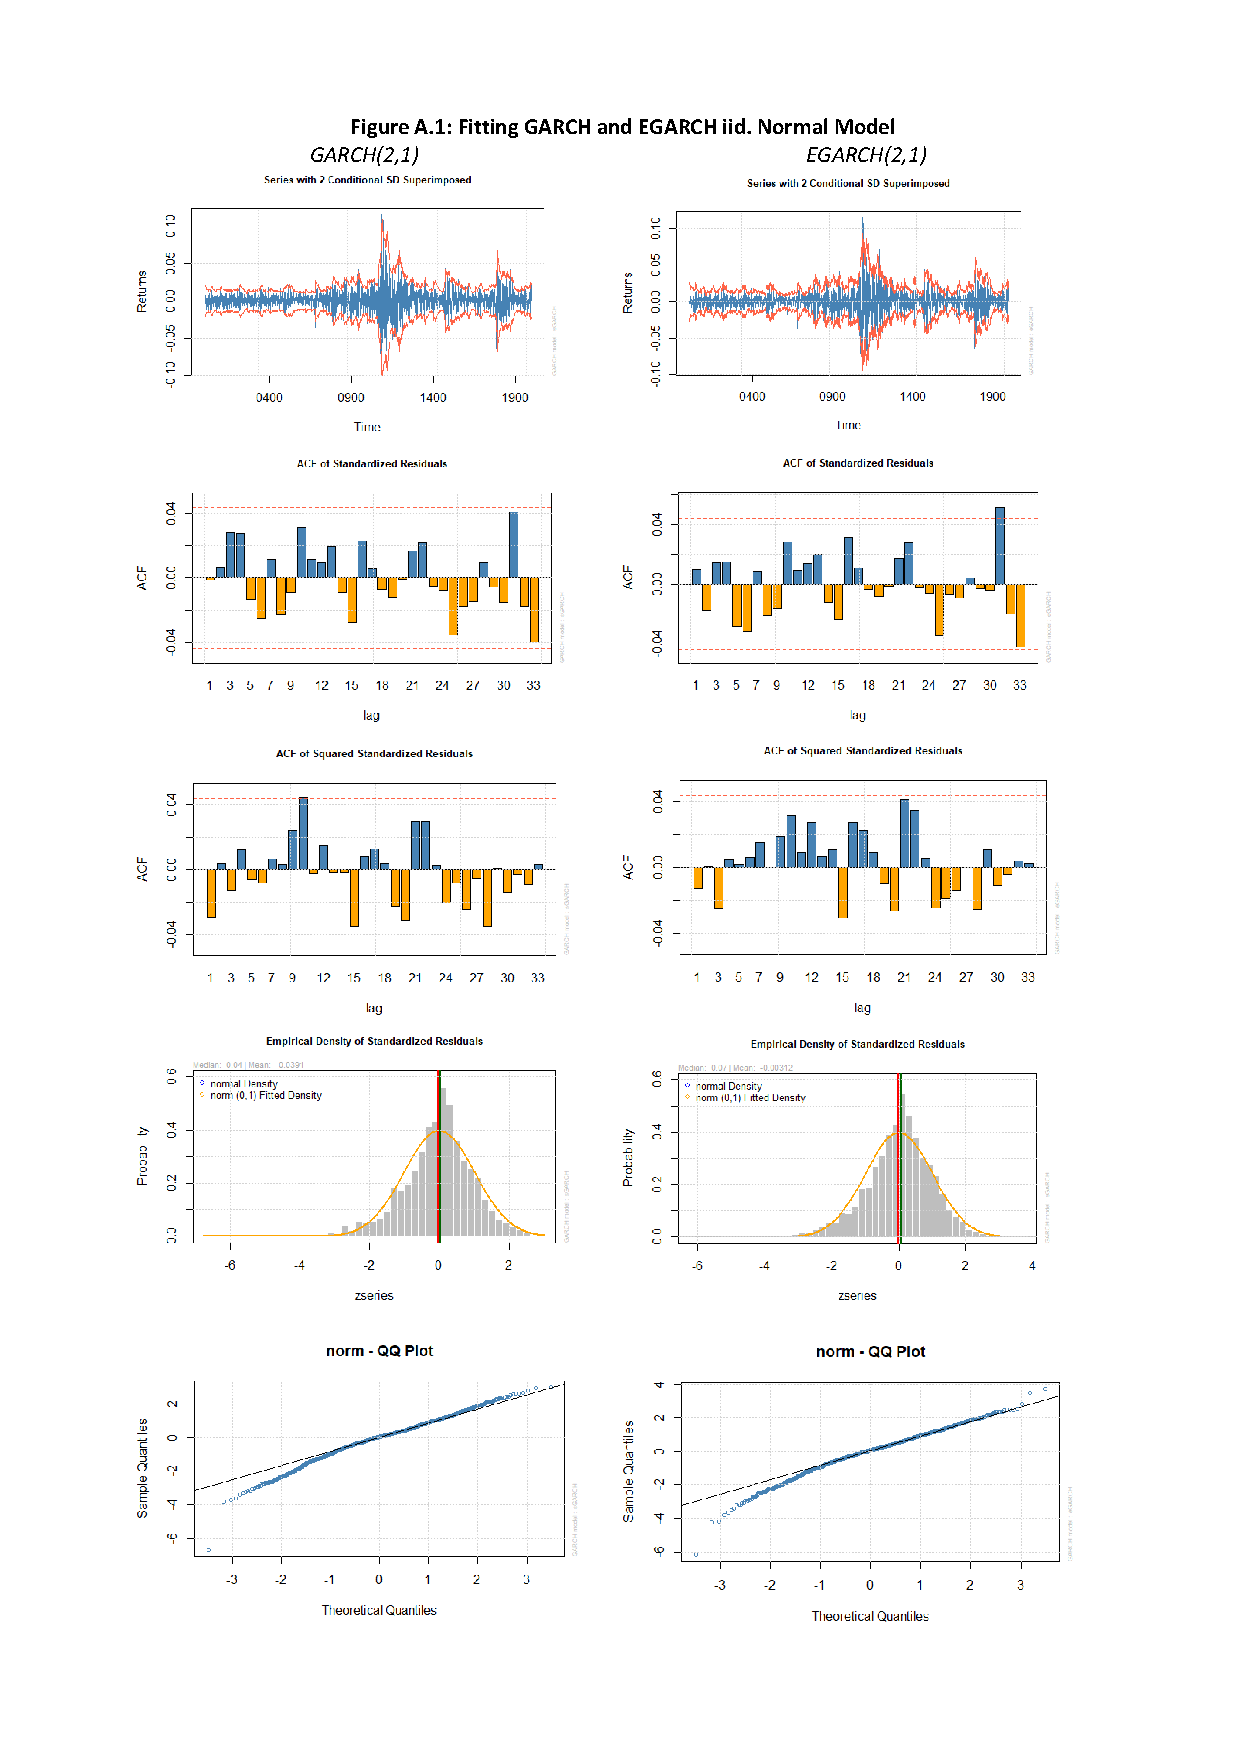
\includepdf[pages=-,pagecommand=\thispagestyle{plain}]{Figure_A1_garch-norm.pdf}
% A2. Std fit 
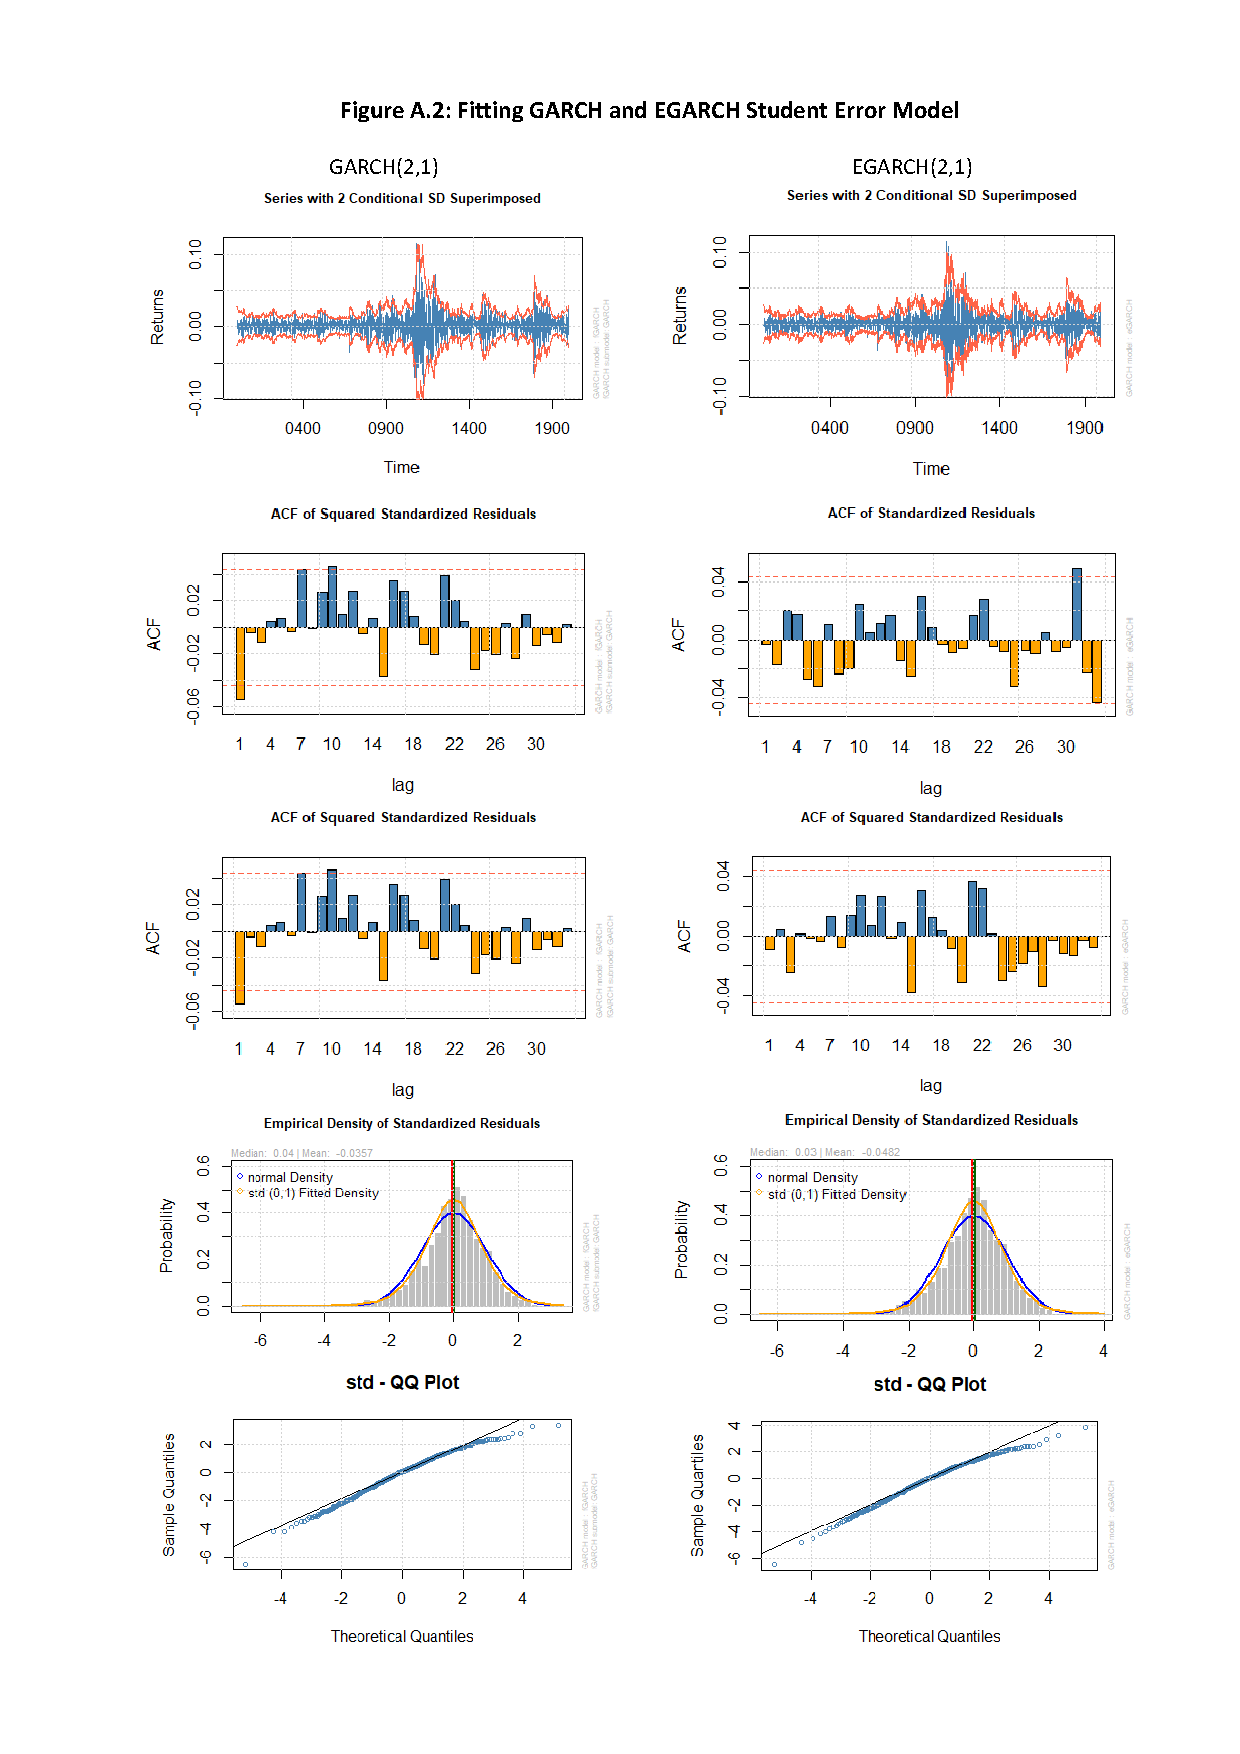
\includepdf[pages=-,pagecommand=\thispagestyle{plain}]{Figure_A2_garch-std.pdf}
% A3. Ged Fit
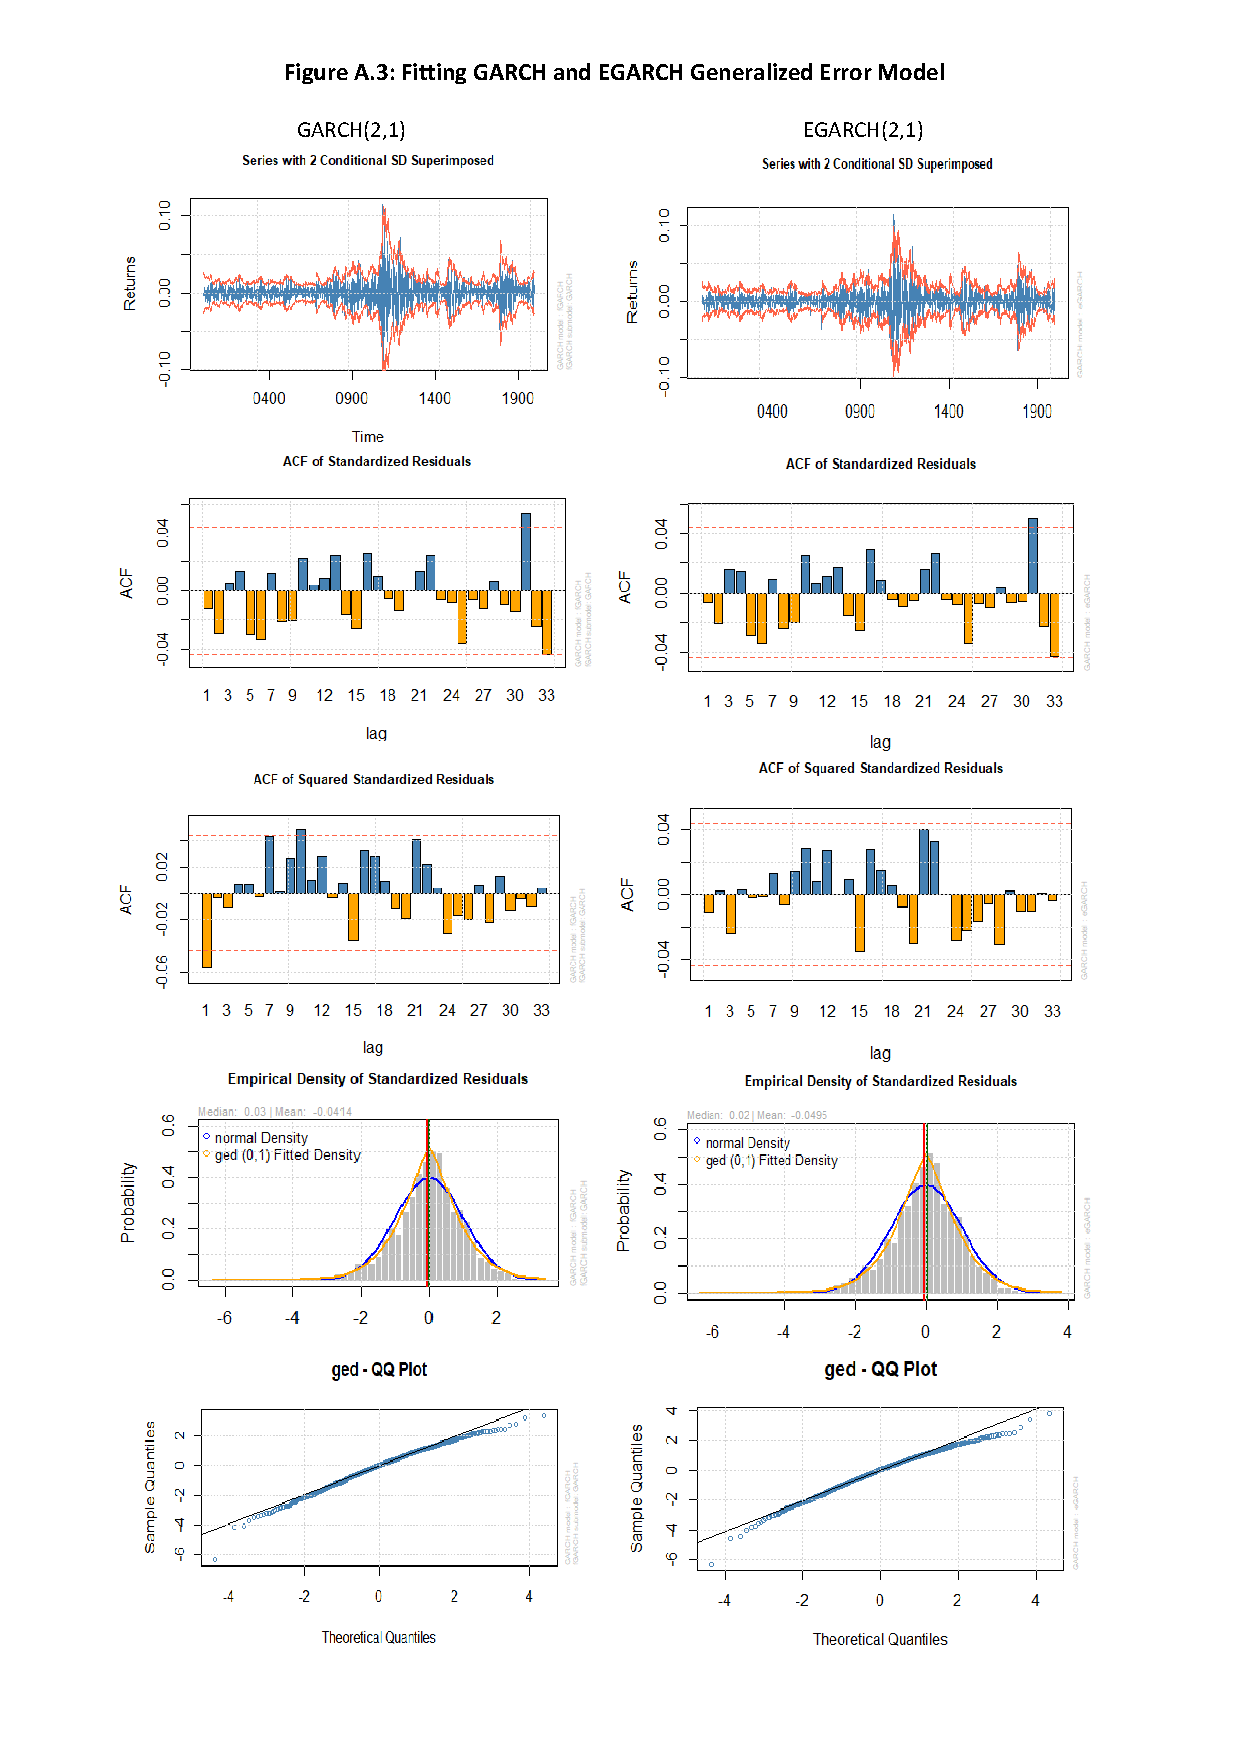
\includepdf[pages=-,pagecommand=\thispagestyle{plain}]{Figure_A3_garch-ged.pdf}
% A4. Norm-Stud Forecast
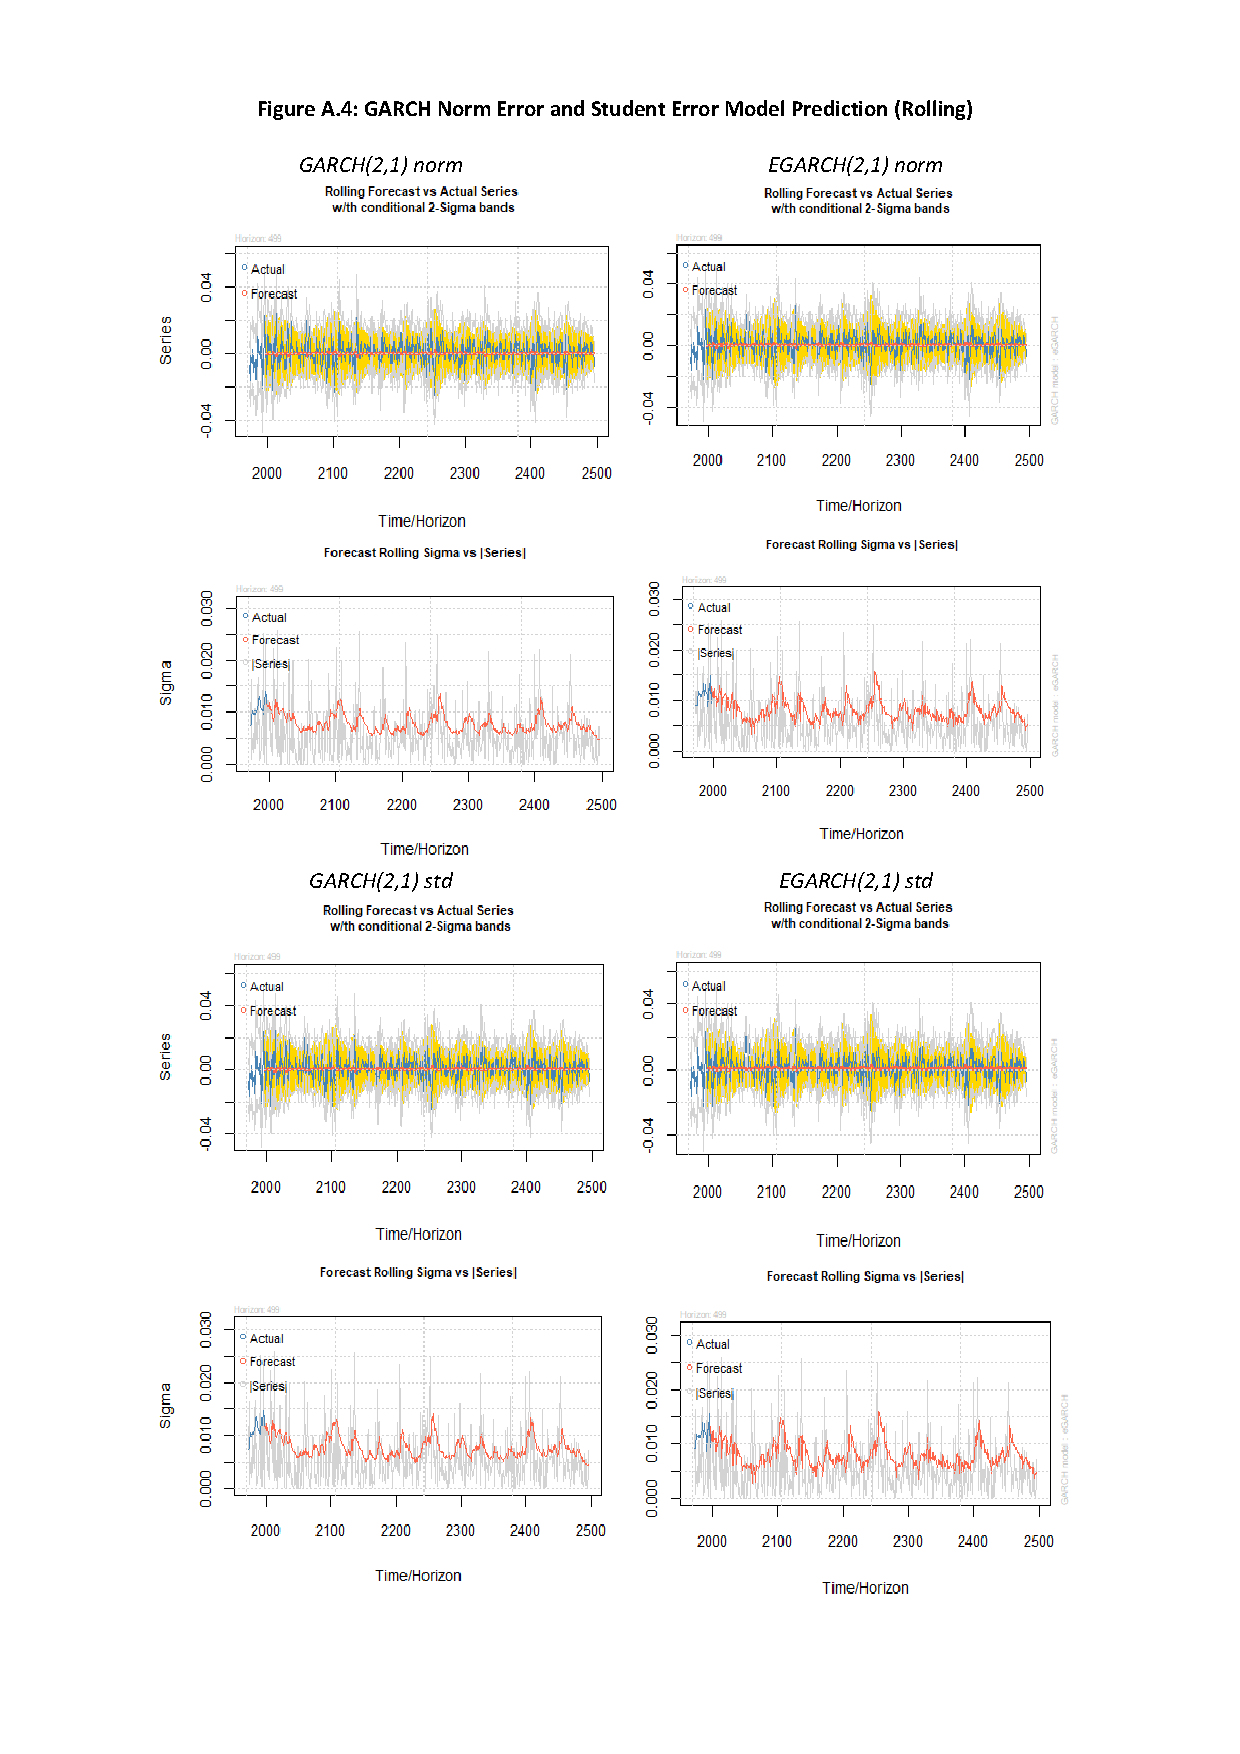
\includepdf[pages=-,pagecommand=\thispagestyle{plain}]{Figure_A4_forecast_std_norm.pdf}
% A5. VaR outsample
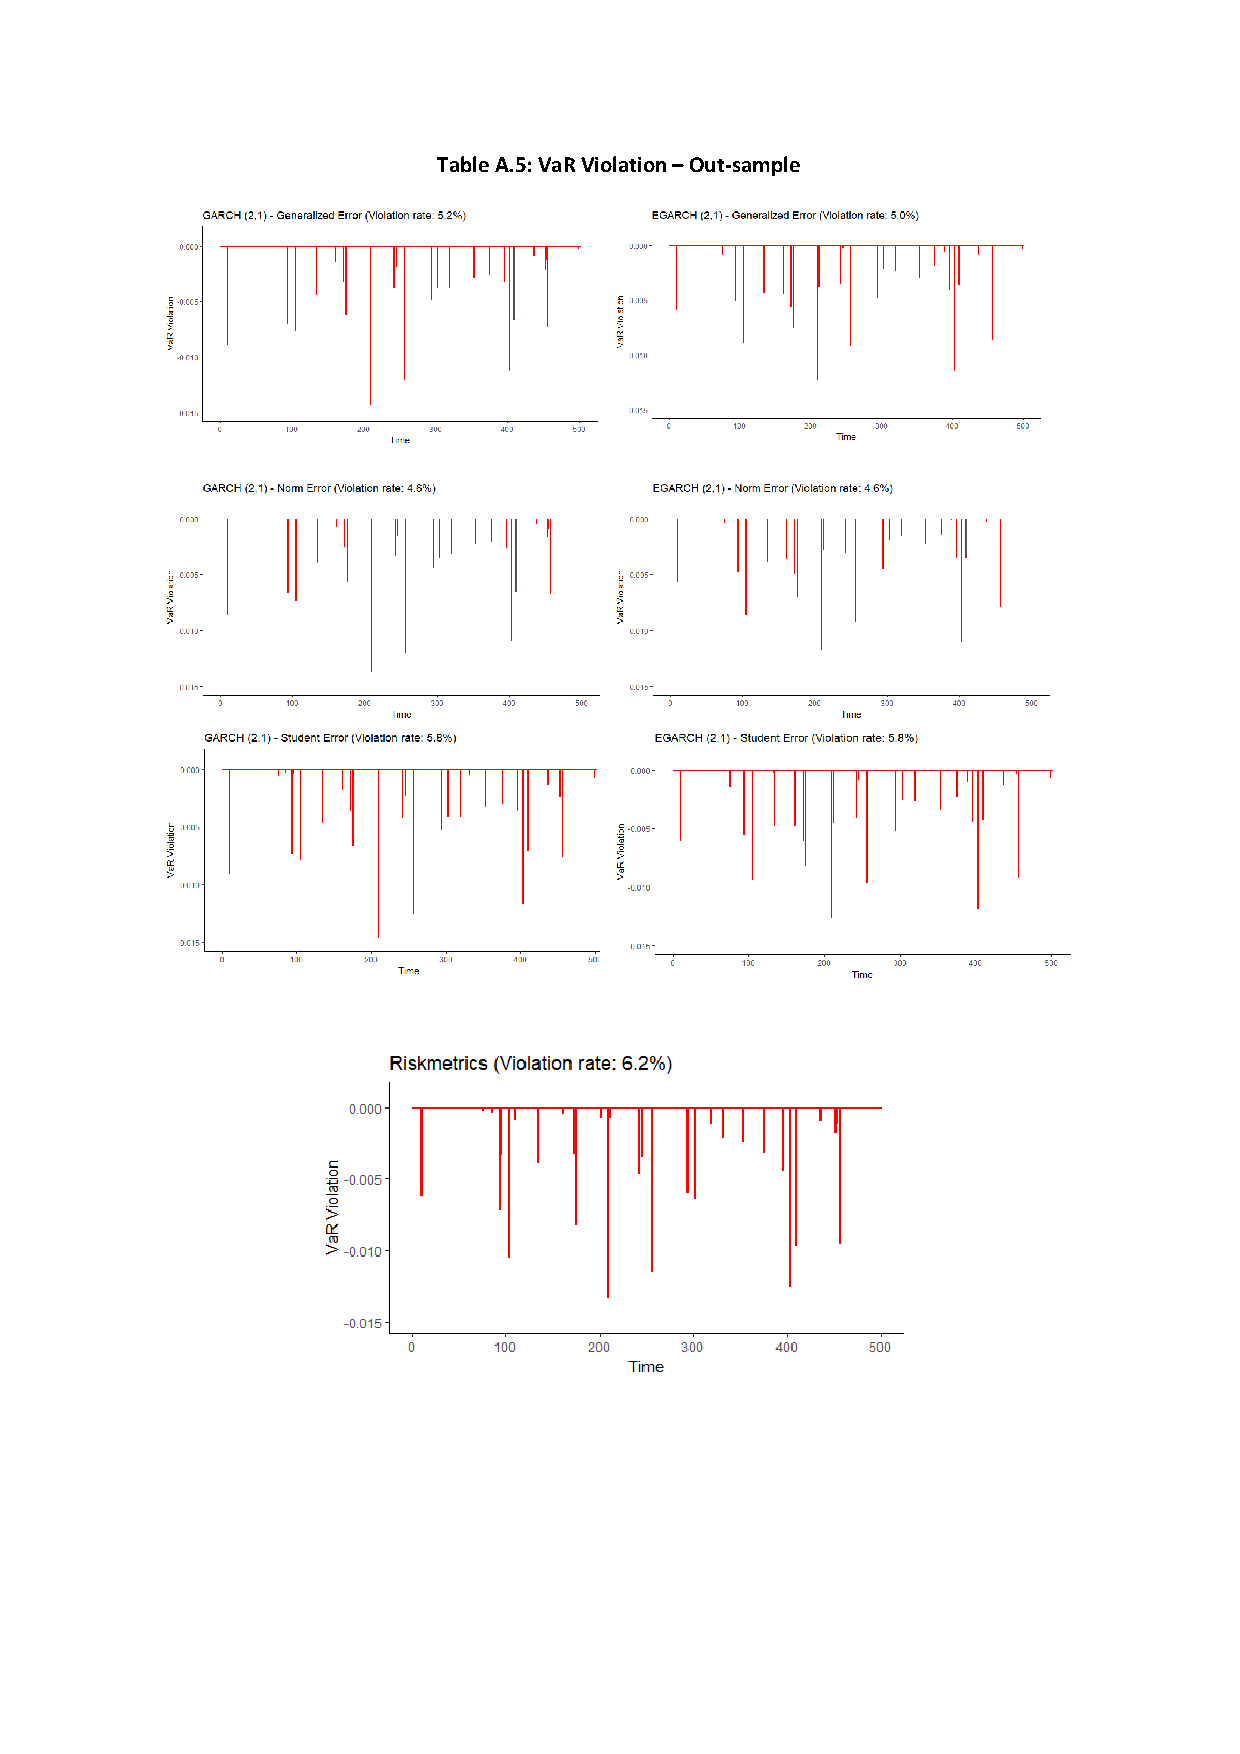
\includepdf[pages=-,pagecommand=\thispagestyle{plain}]{TableA5_var_outsample.pdf}
% A6. News Curve
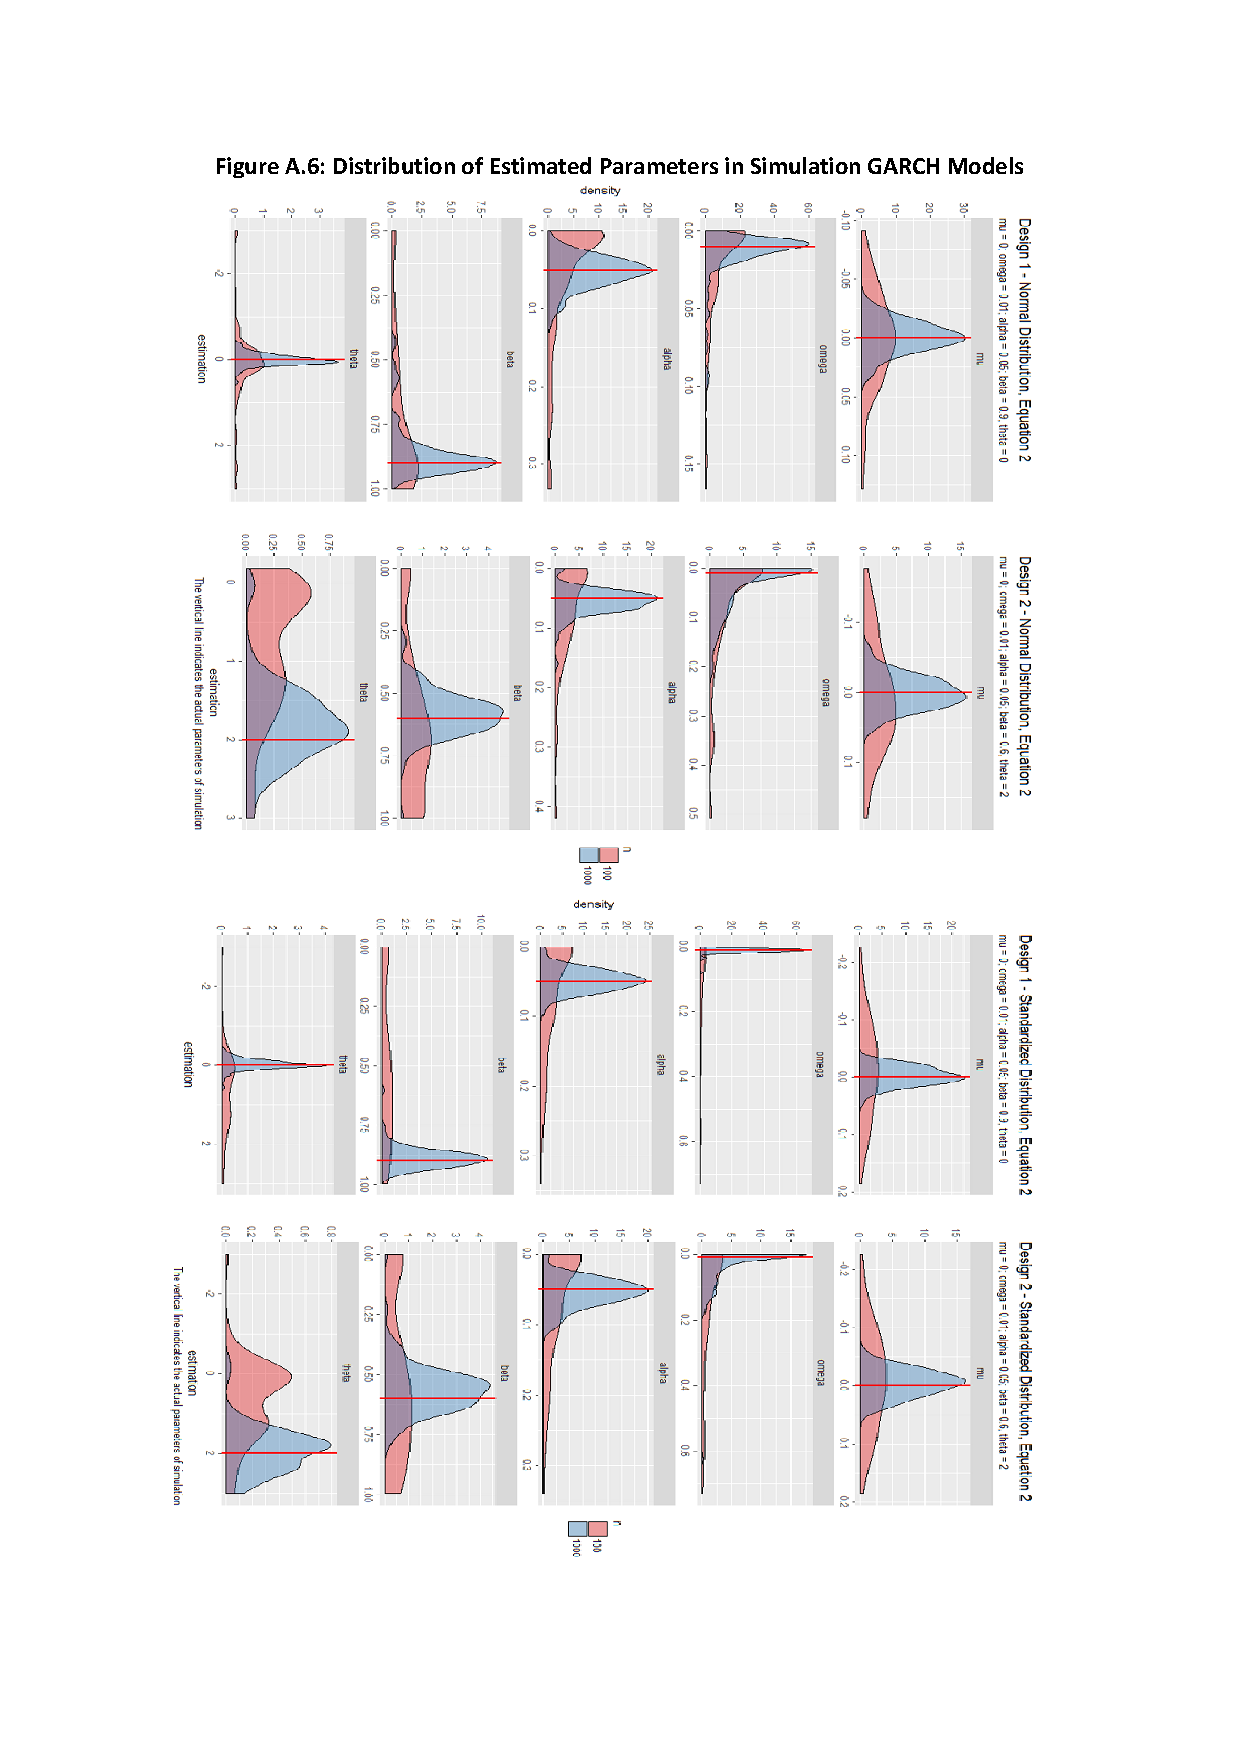
\includepdf[pages=-,pagecommand=\thispagestyle{plain}]{Figure_A6_simulated_dist.pdf}


\end{document}